
\documentclass[12pt]{article}
\usepackage{amssymb}
\usepackage{amsmath}
\usepackage{tikz}

\newtheorem{theorem}{Theorem}


\begin{document}

\title{Trying to converge to an equilibrium flow}
\maketitle

Throughout, Vickrey queuing model is used.

\section*{Iterative Model}

TBD

$$ h_P^{(i+1)}(\theta) = \left(1 - \alpha( d_P^{(i)}(\theta)) \right) \cdot h_P^{i}(\theta) + \frac{ \mathbb{I}_{ \{d_P^{(i)} < \varepsilon \}} (\theta) }{\sum_{P'} \mathbb{I}_{ \{d_{P'}^{(i)} < \varepsilon \}} (\theta)} \cdot \left( \sum_{P'} \alpha( d_P^{(i)}(\theta)) \cdot h_P^{i}(\theta) \right).$$

%\sum_{} \mathbb{I}_{d_P^{i}(\theta) < \varepsilon}

\section*{Dynamic Replicator Model}

Let $\mathcal{P}$ be a collection of $s$-$t$ paths. At time $\theta$, each path $P$ receives a fraction $h_P(\theta)$ of the total inflow $u(\theta)$. We are considering the replication dynamic: 

$$ \dot{h}_P = R \cdot h_P \cdot a_P, \quad ~\forall P \in \mathcal{P}, $$
where $R > 0$ is a constant, $a_P = \phi_P - \sum_{P' \in \mathcal{P}} h_{P'} \cdot \phi_{P'}$ is advantage function based on fitness $\phi$. 

 Role of the fitness can be played by negative signed average experienced travel time of the particles:
%($\theta_l = \max( \theta - w, 0 )$)
$$ \phi^{a.t.}_P(\theta, h) = - \frac{1} {F_P^+(\theta)} \left( \int_{0}^{\theta} F_P^+(\psi) d \psi - \int_{0}^{\theta} F_P^{-} (\psi) d \psi \right) .$$
Above, $F_P^+(\cdot)$, $F_P^-(\cdot)$ denote functions of accumulated path in- and outflow.

Another option is  negative signed last available travel time:
$$ \phi^{l.t.}_P(\theta, h) = -1 \cdot \begin{cases} \theta, & 0 \leq \theta < T_P(0) \\ \theta - T_P^{-1}(\theta), & \theta \geq T_P(0) \end{cases} ,$$
 $T_P(\cdot)$ is path exit time function.
 
Finally, utilising constant predictors for queues, one can predict path exit times $ \hat{T}_P $ and use negative predicted travel time:
$$ \phi^{p.t.}_P(\theta, h) = - (\hat{T}_P(\theta) - \theta) .$$
If path $P$ has only one edge, then $ \hat{T}_P(\cdot) \equiv T_P(\cdot) $.

\subsection*{Considered Instance}

Consider simple network with two parallel edges on Figure \ref{fig:instance}. Let upper edge have index $0$ and lower $1$. We consider inflow $u(\theta) \equiv U$.

\begin{figure}
	\begin{center}
		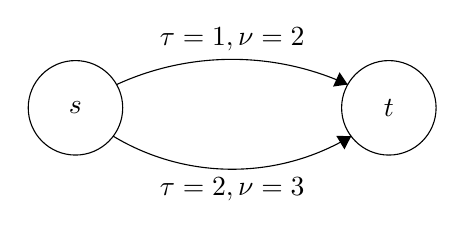
\begin{tikzpicture}[scale=0.2]
			\tikzstyle{every node}+=[inner sep=0pt]
			\draw [black] (7.2,-8.7) circle (3);
			\draw (7.2,-8.7) node {$s$};
			\draw [black] (27.1,-8.7) circle (3);
			\draw (27.1,-8.7) node {$t$};
			\draw [black] (9.808,-7.224) arc (114.62656:65.37344:17.62);
			\fill [black] (24.49,-7.22) -- (23.97,-6.44) -- (23.56,-7.35);
			\draw (17.15,-5.12) node [above] {$\tau=1, \nu=2$};
			\draw [black] (24.706,-10.5) arc (-58.92949:-121.07051:14.642);
			\fill [black] (24.71,-10.5) -- (23.76,-10.48) -- (24.28,-11.34);
			\draw (17.15,-13.1) node [below] {$\tau=2, \nu=3$};
		\end{tikzpicture}
	\end{center}
	\caption{Simple network}
	\label{fig:instance}
\end{figure}

The equilibrium flow is achieved as follows: all the inflow is redirected to the shorter edge, until both edges achieve equal costs, then the distribution is proportional to the capacities.
$$ h^*_0(\theta) = \begin{cases} 1, & 0 \leq \theta < (\tau_1 - \tau_0) \frac{\nu_0}{U - \nu_0} \\  \frac{\nu_0}{U}, &\theta \geq (\tau_1 - \tau_0) \frac{\nu_0}{U - \nu_0} \end{cases}, \quad h^*_1(\theta) = 1 - h^*_0(\theta) .$$


\subsection*{Numerical Approximation}

 show numerically computed inflow shares and fitness of replicator flow with initial condition $h_0(0) = h_1(0) = \frac{1}{2}$. The following approximation was used:

$$ h_P(\theta + \Delta\theta) \approx \frac{ h_P(\theta) \cdot e^{ R \cdot a_P \cdot \Delta \theta }} { \sum_{P'}  h_{P'}(\theta) \cdot e^{ R \cdot a_{P'} \cdot \Delta\theta } } .$$

By construction of the initial dynamic $\sum_{P'}  h_{P'}(\theta) \cdot e^{ R \cdot a_{P'} \cdot \Delta\theta } = 1 + o(\Delta \theta)$. Normalisation is required to remain on simplex.

\newpage

\subsection*{Stabilizing Dynamics (max demand)}

\subsubsection*{Logit Regularization}

One can use modify the fitness using logit regularizer:
	$$ \phi^{\text{reg}}_P(\theta, h) = \phi_P(\theta, h) - \lambda e^{-\gamma \cdot \theta} \ln{ h_P(\theta) }, $$
where $\lambda > 0$ is a scaling constant, $\gamma > 0$ is regularization decay. Figure \ref{fig:reg_pred_tt} shows amplitude drops for different 

\begin{figure}
	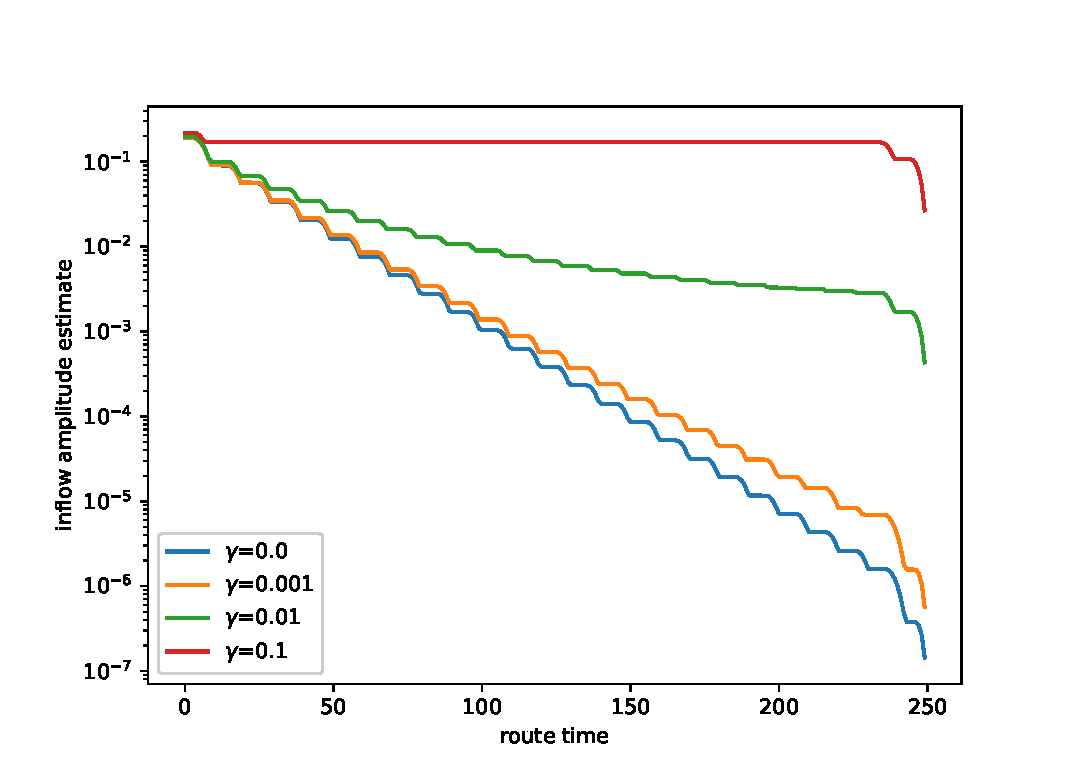
\includegraphics[width=0.9\textwidth]{img/reg_pred_tt.eps}
	\caption{Predicted travel time with logit regularization $\lambda=1$}
	\label{fig:reg_pred_tt}

\end{figure}

\subsubsection*{Projected Travel Times}

If we use projected queue values $\hat{q}^{\delta}_e(\theta') = q_e(\theta) + \frac{q_e(\theta) - q_e(\theta - \delta)}{\delta} \cdot (\theta' - \theta)$ to estimate upcoming travel times, we can use fitness $$ \phi^{\text{proj t.t.}}(\theta, h) = -(t_P(\theta) + w \cdot \frac{\partial t_P}{\partial \theta}(\theta)) \approx - ( \tau_P + \frac{1}{\nu_P} \hat{q}^{\delta}_e(\theta + w) ). $$  Projection window $w$ is a paramater. 

\subsection*{Analysis}
Denote  $\Phi(\theta) := t_0(\theta) - t_1(\theta)$,  $\mathbb{I}_{q_e}(\theta) := \begin{cases} 1, q_e(\theta) > 0 \text{ or } f_e^+(\theta) \geq \nu_e \\ 0, \text{ otherwise}\end{cases}$.
\\
Queue $q_e$ "activates" at the moment $ \theta_{q_e} $ s.t. $f_e^+( \theta_{q_e}) = \nu_e $ and deactivates at first the moment $\theta'_{q_e}$ s.t. $\int_{\theta_{q_e}}^{ \theta'_{q_e}} (f_e^+(z) - \nu_e)  dz  = 0$.
\\
We can write the derivative of $\Phi$ as

 $$ \quad \dot{\Phi} = \left(\frac{U h_0}{\nu_0} - 1 \right) \mathbb{I}_{q_0} - \left(\frac{U (1 - h_0)}{\nu_1} - 1 \right)\mathbb{I}_{q_1} $$
and substitute in replication DE with projected travel times as fitnesses:
 $$ \dot{h_0} = Rh(\phi_0 - h_0\phi_0 -(1-h_0)\phi_1) = Rh_0(1-h_0)(\phi_0 - \phi_1) = -Rh_0(1-h_0)(\Phi + w \dot{\Phi} ) $$
There are 4 different cases:
 \begin{enumerate}
 
	\item $  \mathbb{I}_{q_0} = 1,  \mathbb{I}_{q_1} = 1 $
		
	$$ h_0 = \frac{\dot{\Phi} + \frac{U}{\nu_1}}{\frac{U}{\nu_0} + \frac{U}{\nu_1}} \stackrel{\dot \Phi \to 0}{\to} \frac{\nu_0}{\nu_0 + \nu_1 } =: h^{(1)} . $$

$$ \frac{\ddot{\Phi}}{\frac{U}{\nu_0} + \frac{U}{\nu_1}} = -R \frac{\dot{\Phi} + \frac{U}{\nu_1}}{\frac{U}{\nu_0} + \frac{U}{\nu_1}} \cdot \frac{\frac{U}{\nu_0} - \dot{\Phi}}{\frac{U}{\nu_0} + \frac{U}{\nu_1}} \cdot (\Phi + w \dot{\Phi}) $$

$$ \ddot{\Phi} \approx - k_1 (\Phi + w \dot{\Phi}), \quad k_1 := R \frac{U}{\nu_0 + \nu_1} $$

 
	
	\item  $  \mathbb{I}_{q_0} = 1,  \mathbb{I}_{q_1} = 0 $
	
		$$ h_0 = \frac{\dot{\Phi} + 1}{\frac{U}{\nu_0}} \stackrel{\dot \Phi \to 0}{\to} \frac{\nu_0}{U}  =: h^{(2)} . $$

$$ \frac{\ddot{\Phi}}{\frac{U}{\nu_0} } = -R \frac{\dot{\Phi} + 1}{\frac{U}{\nu_0} } \cdot \frac{\frac{U}{\nu_0} - 1 - \dot{\Phi}}{{\frac{U}{\nu_0} }} \cdot (\Phi + w \dot{\Phi}) $$

$$ \ddot{\Phi} \approx - k_2 (\Phi + w \dot{\Phi}), \quad k_2 := R( 1 -\frac{\nu_0}{U}) $$

	\item  $  \mathbb{I}_{q_0} = 0,  \mathbb{I}_{q_1} = 1 $
	
		$$ h_0 = \frac{\dot{\Phi} + \frac{U}{\nu_1} - 1}{\frac{U}{\nu_1}} \stackrel{\dot \Phi \to 0}{\to} \frac{U - \nu_1}{U}  =: h^{(3)} . $$

$$ \frac{\ddot{\Phi}}{\frac{U}{\nu_1} } = -R \frac{\dot{\Phi} + \frac{U}{\nu_1} - 1}{\frac{U}{\nu_1}} \cdot \frac{ 1 - \dot{\Phi}}{{\frac{U}{\nu_1} }} \cdot (\Phi + w \dot{\Phi}) $$

$$ \ddot{\Phi} \approx - k_3 (\Phi + w \dot{\Phi}), \quad k_3 := R( 1 -\frac{\nu_1}{U}) $$

	\item  $  \mathbb{I}_{q_0} = 0,  \mathbb{I}_{q_1} = 0 $ 
	
	$$ \frac{d}{d\theta} \ln \frac{h_0}{1-h_0} = \frac{\dot{h_0}}{h_0 (1-h_0)} = R(\tau_1 - \tau_0)$$
	
	$$ h_0(\theta) = \sigma \left( \ln \frac{h_0(\theta_0)}{1 - h_0(\theta_0)} + R(\tau_1 - \tau_0)(\theta - \theta_0) \right) \stackrel{\theta \to  \infty}{\to} 1, \quad \sigma(x) = \frac{1}{1 + e^{-x}}$$
 
 \end{enumerate}

For equation $\ddot{\Phi} + k (\Phi + w \dot{\Phi}) = 0$ we can estimate the solution decay rate:
$$ w \leq \frac{2}{\sqrt{k}}: \quad t_0 - t_1, h_0 - h^* \propto e^{-\frac{kw}{2} \theta}$$ 
$$w > \frac{2}{\sqrt{k}}: \quad t_0 - t_1, h_0 - h^* \propto e^{-\frac{kw - \sqrt{(kw)^2 - 4k}}{2}\theta}$$

\subsubsection*{Case switching}

We have invariants $\Phi$, and $h_0$. Below we study the derivative switch $ \dot{\Phi} \to \dot{\Phi'} $. 

\begin{itemize}

	\item $1 \to 2$. Necessary conditions: $h_0 > 1 - \frac{\nu_1}{U}$, $\Phi = \Phi' \geq \tau_0 - \tau_1$.
$$ \frac{\dot{\Phi} + \frac{U}{\nu_1}}{\frac{U}{\nu_0} + \frac{U}{\nu_1}} = \frac{\dot{\Phi'} + 1}{\frac{U}{\nu_0}}$$		
$$ \dot{\Phi'} = \frac{\dot{\Phi} - \frac{ \nu_0 + \nu_1 - U }{\nu_1} }{\frac{\nu_0 + \nu_1}{\nu_1}} $$
We are either close to equilibrium, or decrease $|\dot{\Phi}|$:
$$  |\dot{\Phi |} < \frac{\nu_0 + \nu_1 - U}{\nu_0} \quad \Rightarrow \quad  | \dot{\Phi'}| < \frac{\nu_0 + \nu_1 - U}{\nu_0} $$
$$ \dot{\Phi} \geq \frac{\nu_0 + \nu_1 - U}{\nu_0}  \quad \Rightarrow \quad |\dot{\Phi'}| \leq |\dot{\Phi}| $$

	\item $1 \to 3$. Necessary conditions: $h_0 < \frac{\nu_0}{U}$, $\Phi = \Phi' \leq \tau_0 - \tau_1$.
$$  \frac{\dot{\Phi} + \frac{U}{\nu_1}}{\frac{U}{\nu_0} + \frac{U}{\nu_1}} = \frac{\dot{\Phi'} + \frac{U}{\nu_1} - 1}{\frac{U}{\nu_1}} $$
$$ \dot{\Phi'} = \frac{ \dot{\Phi} + \frac{\nu_0 + \nu_1 - U}{\nu_0} }{ \frac{\nu_0 + \nu_1}{\nu_0} } $$
 We are either close to equilibrium, or decrease $|\dot{\Phi}|$:
$$ |\dot{\Phi}| < \frac{\nu_0 + \nu_1 - U}{\nu_1} \quad \Rightarrow \quad |\dot{\Phi'}| < \frac{\nu_0 + \nu_1 - U}{\nu_1}$$

$$ \dot{\Phi} < - \frac{\nu_0 + \nu_1 - U}{\nu_1} \quad \Rightarrow \quad |\dot{\Phi'}| < |\dot{\Phi}|$$

	\item $2 \to 1$. Necessary condition: $h_0 = 1 - \frac{\nu_1}{U}$.
$$     \frac{\dot{\Phi} + 1}{\frac{U}{\nu_0}} = \frac{\dot{\Phi'} + \frac{U}{\nu_1}}{\frac{U}{\nu_0} + \frac{U}{\nu_1}} = 1 - \frac{\nu_1}{U} $$
 $$ \dot{\Phi}= \dot{\Phi'} = - \frac{\nu_0 + \nu_1 - U}{\nu_0}$$

	\item $3 \to 1$. Necessary condition: $h_0 = \frac{\nu_0}{U}$.
$$ \frac{ \dot{\Phi} + \frac{U}{\nu_1} - 1}{\frac{U}{\nu_1}} = \frac{\dot{\Phi'} + \frac{U}{\nu_1}}{\frac{U}{\nu_0} + \frac{U}{\nu_1}} = \frac{\nu_0}{U} $$
$$ \dot{\Phi}= \dot{\Phi'} = \frac{\nu_0 + \nu_1 - U}{\nu_1}$$


	\item $ 2 \to 4 \to 2$. Necessary conditions: $h_0 < \frac{\nu_0}{U}$, $\Phi = \Phi' = \tau_0 -\tau_1 < 0 $ .
	\\
	$$ \dot{\Phi} < 0 , ~\dot{\Phi'} = 0 \quad \Rightarrow \quad |\Phi' + w\dot{\Phi'}| < |\Phi + w\dot{\Phi}| . $$

\item $ 3 \to 4 \to 2$. Necessary conditions: $ 1 - \frac{\nu_1}{U} < h_0 < \frac{\nu_0}{U}$, $\Phi = \Phi' = \tau_0 -\tau_1 < 0 $ .
	\\
	$$ 0 < \dot{\Phi} < \frac{\nu_0 + \nu_1 - U}{\nu_1} , ~\dot{\Phi'} = 0 . $$


\end{itemize}

\newpage

\subsection*{Mupltiple links}

Consider $n$ parallel links $\{(\tau_i, \nu_i)\}_{i=1}^n$ with strict ordering of travel times $\tau_1 < \dots < \tau_n$ and demand $\nu_1 < U < \sum_{i} \nu_i$. 

$$ \dot{h_i} = R h_i( \phi_i - \sum_{j=1}^n h_j \phi_j ) = R h_i(1-h_i) \left( 
\phi_i - \overline{\phi_{-i}} \right) , \quad i = 1 \dots n $$
$$ \overline{\phi_{-i}} := \sum_{j \neq i} \frac{h_j}{\sum_{j' \neq i} h_{j'}} \phi_j  $$
Where we use negative projected travel times as fitnesses:
$$ \phi_i = - ( t_i + w \dot{t_i}) = -\left( \tau_i + \frac{q_i}{\nu_i} + w \cdot \left( \frac{Uh_i}{\nu_i} - 1 \right) \mathbb{I}_{q_i} \right) .$$
Suppose there exists $k^* \leq n$, s.t.
$$ \sum_{i=1}^{k^*-1} \nu_i < U < \sum_{i=1}^{k^*} \nu_i .$$
Then one can show the following state is the equilibrium:
$$ \mathbb{I}_{q_i} = \mathbb{I}_{[ i < k^* ]};  \quad t^*_i := \begin{cases} \tau_{k^*}, ~i \leq k^* \\ \tau_i, ~i > k^*  \end{cases}; \quad h^*_i = \begin{cases} \frac{\nu_i}{U}, i < k^* \\ 1 - \sum_{i < k^*} h^*_{i}, ~ i = k^*\\  0, ~i > k^*  \end{cases}. $$



%First show for $k^* = n$, then try to generalize
%$$ h_{> k^*} := \sum_{j > k^*} h_j; \quad \phi_{>k^*} := \sum_{j > k^*} \frac{h_j}{  h_{> k^*}  } \phi_j $$

Assuming same queue configuration, we can linearize the system near the equillibrium. Below, we denote $\Delta h := h - h^*$, $\Delta t := t - t^*$.
$$ \dot{ \Delta h_i} \approx -Rh^*_i \left( \left( \Delta t_i + \frac{w }{h^*_i} \Delta h_i \right) - \sum_{j < k^*} h^*_j \left( \Delta t_j + \frac{w }{h^*_j} \Delta h_j \right)  - \sum_{j > k^*} \Delta h_j \tau_j \right), ~i < k^*$$
$$ \dot{ \Delta h_{k^*}} \approx -R h^*_{k^*} \left( 0 - \sum_{j < k^*} h^*_j \left( \Delta t_j + \frac{w }{h^*_j} \Delta h_j \right) - \sum_{j > k^*} \Delta h_j \tau_j \right) $$
$$ \dot{\Delta h_i} \approx -R \Delta h_i( \tau_i - \tau_{k^*}), ~i > k^* $$
$$ \dot{\Delta t_i} = \frac{1}{h^*_i} \Delta h_i, ~ i < k^*; \quad \dot{\Delta t_i} = 0, ~ i \geq k^*$$

$$ \frac{d}{d \theta} \begin{bmatrix} \Delta h_{< k^*} \\ \Delta t_{< k^*} \\ \Delta h_{k*} \\ \Delta t_{k^*} \\ \Delta h_{> k^*} \\ \Delta t_{> k^*} \end{bmatrix} \approx 
-R A
 \begin{bmatrix} \Delta h_{< k^*} \\ \Delta t_{< k^*} \\ \Delta h_{k*} \\ \Delta t_{k^*} \\ \Delta h_{> k^*} \\ \Delta t_{> k^*} \end{bmatrix} ,$$
 $$ A  = \begin{bmatrix} 
 w(I - h^*_{< k^*} \textbf{1}^T) &  h^*_{< k^*} (I - (h^*_{< k^*})^T)  & 0 & - h^*_{< k^*} h^*_{k^*}  & - h^*_{< k^*} \tau_{> k^*}^T & 0 \\
 \frac{1}{h^*_{<k^*}} & 0 & 0  & 0 & 0 & 0 \\
  - h^*_{k^*} w h^*_{< k^*}   & 0 & h^*_{k^*} \tau & b^T & h^*{k^*}(1-h^*{k^*}) & 0 \\ 
 0 & 0 & 0 & 0 & 0 & 0 \\ 
\frac{w}{h^*} I & 0 & 0 & 0 & 0 & 0 \\
0 & 0 & 0 & 0 &  (\tau - \tau_{k^*} ) I & 0 \\  \end{bmatrix} $$

\newpage

\subsection*{Lyapunov Theory}
Our differential equation has form $ \ddot{\Phi} = g(\Phi, \dot{\Phi})$, where $g$ is a polynomial. We view it as autnomous system with Lipshitz RHS
$$  \frac{d}{d\theta} \begin{bmatrix} \Phi \\ \dot{\Phi} \end{bmatrix} = \begin{bmatrix} \dot{\Phi} \\ g(\Phi, \dot{\Phi}) \end{bmatrix} $$
In this case Lyapunov Theory is applicable. 
\\
In general, we consider autonomous system
$$ \dot{x} = f(x), \quad f(0) = 0.$$
\begin{theorem}(Global asymptotic stability) 
Let $V: \mathbb{R}^n \to \mathbb{R}$ be a continuously differentiable function, s.t. :
$$V(0) = 0 \text{ and } \forall x \neq 0: ~V(x) > 0  , $$
$$ \lVert x \rVert_2 \to \infty \quad \Rightarrow \quad V(x) \to \infty, $$
$$ \forall x \neq 0 :  ~\dot{V} =  \nabla V(x) \cdot f(x) < 0 $$
Then $x = 0$ is globally asymptotically stable.
\end{theorem}

\begin{theorem}(Local asymptotic stability)
Let $A = \frac{\partial f}{\partial x}(0)$ be Jacobian matrix at $x=0$. If we have $\mathrm{Re} (\lambda_i(A)) < 0$ for all eigenvalues, then $x = 0$ is locally asymptotically stable.

\end{theorem}

\subsubsection*{Local stability}
We consider the linearized equation 
$$\ddot{\Phi} = \frac{\partial f}{\partial \Phi}(0,0) \cdot \Phi + \frac{\partial f}{\partial \dot{\Phi}}(0,0) \cdot \dot{\Phi} = -k\Phi - kw\dot{\Phi} .$$
Searching for eigenvalues yields
$$ \mathrm{det} \left( \begin{bmatrix} -\lambda & 1 \\ -k & -kw - \lambda \end{bmatrix} \right) = \lambda^2 + kw \lambda + k; \quad D = k^2w^2 - 4k. $$
 $ D \geq 0: \quad \mathrm{Re}(\lambda_{1,2}) = -\frac{kw}{2} \pm \sqrt{ \left( \frac{kw}{2} \right)^2  -k } < 0,$
 \\
 $ D < 0: \quad  \mathrm{Re}(\lambda_{1,2}) = -\frac{kw}{2} < 0.$
 \\
Hence, we always have local asymptotic stability.

\subsubsection*{Sufficient conditions for global stability (Quadratic potential)}
In case $i \in \{ 1, 2, 3 \}$ we can write the equation as
$$ \ddot{\Phi} = - RC_i h_0(1-h_0)(\Phi + w \dot{\Phi}).$$ 
Denote 
$$ C := \min_{i \in \{ 1, 2, 3 \}} C_i = \min \left\{  \frac{U}{\nu_0} + \frac{U}{\nu_1} , \frac{U}{\nu_0} , \frac{U}{\nu_1} \right\} = \frac{ U}{\max \{ \nu_0, \nu_1 \}}.$$
%We can bound $ \frac{U}{\nu_0} + \frac{U}{\nu_1} \leq 2\frac{\nu_0 + \nu_1}{\min\{ \nu_0, \nu_1 \}}$
Further, assume that
 $$ \forall \theta \geq 0: \quad h_0(\theta) \in [a, b] \text{ with } a > 0, b < 1$$
  and denote  $m := \min_{x \in [a,b]} x(1-x) > 0 $.
\\
Consider Lyapunov function $V(\Phi, \dot{\Phi}) = \Phi^2 + (\Phi + w \dot{\Phi}) ^2 >0 $.
$$ \dot{V} = \frac{\partial V}{\partial \Phi} \dot{\Phi} + \frac{\partial V}{\partial \dot{\Phi}} \cdot \left( -RC_i  h_0(1-h_0)(\Phi + w \dot{\Phi}) \right)  = $$
$$ = \left( 4\Phi + 2w\dot{\Phi} \right)\dot{\Phi}  - 2w R C_i h_0(1-h_0)(\Phi + w \dot{\Phi})^2 \leq $$
$$ \leq  4\Phi\dot{\Phi} + 2w\dot{\Phi}^2 - 2wRCm (\Phi + w \dot{\Phi})^2 = $$
$$ = 2w \left( \frac{1}{w^2} - RCm \right)  (\Phi + w \dot{\Phi})^2 - \frac{2}{w} \Phi^2  .$$
\\
We can guarantee $\dot{V} < 0$ if $w \geq \frac{1}{\sqrt{RCm}}$.
\\
For $R = 0.1, U = 4.5, [a,b] = [0.01, 0.99]$ we need $w \geq \frac{1}{\sqrt{ 0.1 \cdot \frac{ 4.5}{3} \cdot 0.01 \cdot .99}} \approx 25.95 $.
\\
If we have $V = \Phi^2 + (\Phi + w\dot{\Phi})^2 \leq B^2$, then it follows that $ |\Phi| \leq B $, $ | \dot{\Phi} | \leq \frac{\sqrt{2}B}{w} $.  
\\
Suppose we can reach $V = B^2$ s.t. $\frac{\sqrt{2}B}{w} = \frac{\nu_0 + \nu_1 - U}{\nu_0} $ 
Then we stop case switching?
%
%\newpage
%
%\subsubsection*{Search for V}
%
%Let $ \frac{\partial V}{\partial \Phi} = p(\Phi, \dot{\Phi})$, $ \frac{\partial V}{\partial \dot{\Phi}} = q(\Phi, \dot{\Phi})$. 
%We need these conditions fulfilled:
%$$ \frac{\partial p}{\partial \dot{\Phi}} = \frac{\partial q}{\partial \Phi}, \quad \begin{bmatrix} \frac{\partial p }{\partial \Phi} &  \frac{\partial p }{\partial \dot{\Phi}} \\  \frac{\partial q }{\partial \Phi} &  \frac{\partial q }{\partial \dot{\Phi}} \end{bmatrix} \succeq 0 $$
%$$ \dot{V} = p \cdot \dot{\Phi} - q \cdot RC_ih(1-h)(\Phi + w \dot{\Phi}) < 0 $$
%Quadratic V: 
%%$$ V = 2\alpha \Phi^2 + \Phi\dot{\Phi} + 2\gamma \dot{\Phi}^2 $$
%$$ p =  \alpha \Phi + \dot{\Phi}; \quad q = \Phi + \gamma \dot{\Phi}; \quad (\alpha, \gamma) \in \{ (\alpha, \gamma) \in \mathbb{R}^2_{>0} | ~ \alpha \gamma - 1 > 0  \} =: G. $$
%$$ -\dot{V} = RC_ih_0(1-h_0) ( \Phi^2 + ( w + \gamma) \Phi\dot{\Phi} + \gamma w \dot{\Phi}^2) - \alpha \Phi \dot{\Phi} - \dot{\Phi} ^2 $$
%We need the following matrix be positive semi-definite for any \\ $K \in \{  \frac{1}{RC_i h (1-h)} | ~i \in \{1,2,3\}; ~ h \in [a,b] \} =: \mathcal{K} \subseteq [\frac{4}{R C_1}, \frac{1}{R C m} ]$:
%$$ \begin{bmatrix}
%	1 & ( w + \gamma - \alpha K )/2 \\
%	( w + \gamma - \alpha K )/2  &  \gamma w - K
%\end{bmatrix} \succeq 0 $$
%Hence, we need to find $(\alpha, \gamma ) \in G$ s.t.
%$$ \inf_{ K \in \mathcal{K} } 4 ( \gamma w -  K ) - ( w + \gamma - \alpha K  )^2  > 0 $$
%Since the function is quadratic, it sufficies to have $ \Delta > 0 $ for  $K \in \left \{ \frac{4}{R C_1}, \frac{1}{R C m} \right\} $. 
%$$  4  ( \gamma w -  K ) - ( w + \gamma - \alpha K  )^2 = (  \alpha K  + w)^2 - (\alpha K - w)^2 - 4K - ( \gamma - w - \alpha K )^2 = $$
%$$ =  4K(\alpha w - 1) - ( \gamma - w - \alpha K )^2  $$
%$$ \Delta = 0 \quad \Rightarrow \quad \gamma = w + \alpha K \pm 2 \sqrt{K(\alpha w -1)} = 1/\alpha + \left( \sqrt{\alpha K} \pm \sqrt{ w - 1/\alpha } \right)^2$$
%The larger root for $K = \frac{4}{R C_1}$ should be larger than smaller root for $K = \frac{1}{R C m}$:
%$$ \sqrt{\alpha \cdot \frac{4}{R C_1} } + \sqrt{ w - 1/\alpha } > \sqrt{\alpha \cdot \frac{1}{R C m} } - \sqrt{ w - 1/\alpha }$$
%$$ 2\sqrt{ 1/\alpha (w - 1/\alpha) } > \sqrt{\frac{1}{R C m} } -  \sqrt{\frac{4}{R C_1} }$$
%LHS is maximized by $\alpha = 2/w$. The final condition is
%$$ w > \sqrt{\frac{1}{R C m} } -  \sqrt{\frac{4}{R C_1} } $$
%For $R = 0.1, U = 4.5, [a,b] = [0.01, 0.99]$ that is 
%$$ w >  \frac{1}{\sqrt{ 0.1 \cdot \frac{ 4.5}{3} \cdot 0.01 \cdot 0.99}} -  \frac{2}{\sqrt{ 0.1 \cdot (\frac{ 4.5}{2} + \frac{ 4.5}{3}  )  }}  \approx 25.95 - 3.26 = 22.68$$
%The choice of parameters:
%$$ \alpha = \frac{2}{w}, \quad \gamma = \frac{w}{2} + \frac{1}{2w} \left( \sqrt{\frac{1}{R C m} } + \sqrt{\frac{4}{R C_1} } \right)^2 .$$


\newpage

\subsection*{Inflow potentials}
Having the functional relation
$$ \dot{\Phi}(h_0) = \left(\frac{U h_0}{\nu_0} - 1 \right) \mathbb{I}_{q_0} - \left(\frac{U (1 - h_0)}{\nu_1} - 1 \right)\mathbb{I}_{q_1} = C_i(h_0 - h^{(i)}),$$
we can construct the Lyapunov function
$$ V(\Phi, \dot{\Phi}) = \frac{1}{2} \Phi^2 + \frac{1}{R} \int_{\dot{\Phi}(h) = 0}^{h_0} \frac{\dot{\Phi}(h) dh}{h(1-h)} = \frac{1}{2} \Phi^2 + \frac{1}{R} \int_{h^{(i)}}^{h_0} \frac{C_i(h - h^{(i)}) }{h(1-h)} dh> 0.$$
Then, for each case $i = 1,2,3$ we have
$$ \dot{V} = \Phi \cdot \dot{\Phi} - \frac{ \dot{\Phi }}{R C_i h_0(1-h_0)} \cdot RC_i h_0(1-h_0) (\Phi + w\dot{\Phi}) = -w \dot{\Phi}^2 < 0$$
The integral can be computed:
$$ \int \frac{ C_i(h_0 - h^{(i)}) dh_0}{h_0(1-h_0)} = C_i \left( \ln \frac{1}{1-h_0} - h^{(i)} \ln \frac{h_0}{1-h_0} \right) + \mathrm{const} $$
We introduce inflow potentials for the cases 2 and 3
$$ \Pi_0 := \int_{ \frac{\nu_0}{U} }^{h_0} \frac{\frac{U}{\nu_0}(h - \frac{\nu_0}{U})}{h(1-h)} dh, \quad  \Pi_1 := \int_{ \frac{U - \nu_1}{U} }^{h_0} \frac{\frac{U}{\nu_1}(h - \frac{U - \nu_1}{U})}{h(1-h)} dh. $$
One can observe that their sum plays a role of potential in the case 1
$$ \Pi_0 + \Pi_1 = \int_{\frac{\nu_0}{\nu_0 + \nu_1}}^{h_0} \frac{(\frac{U}{\nu_0} + \frac{U}{\nu_1})(h - \frac{\nu_0}{\nu_0 + \nu_1})}{h(1-h)} dh + \Delta \Pi, $$
where we have a constant
$$ \Delta \Pi:= \int_{\frac{\nu_0}{\nu_0 + \nu_1}}^{\frac{\nu_0}{U}} \frac{\frac{U}{\nu_0}( \frac{\nu_0}{U} - h)}{h(1-h)} dh + \int_{\frac{U - \nu_1}{U}}^{\frac{\nu_0}{\nu_0 + \nu_1}} \frac{\frac{U}{\nu_1}(h - \frac{U - \nu_1}{U})}{h(1-h)} dh \geq 0,$$
with property $\Delta \Pi =0 \Leftrightarrow U = \nu_0 + \nu_1$.
\\
Hence, function $V = \frac{1}{2} \Phi^2 + \Pi_0 \mathbb{I}_{q_0} + \Pi_1 \mathbb{I}_{q_1}$ has following propreties:
\begin{itemize}
	\item $V = 0$ only at the equillibrium, else $V > 0$;
	\item $V \to \infty$ if $|\Phi| \to \infty$ or $h_0 \to 0,1$;
	\item $ \dot{V} < 0 $ during the cases $1,2,3$.
\end{itemize}
There still remain a problem of case switching. Namely, we need to show that  particular case switches (e.g.  $2 \to 1 \to 2$, $2 \to 1 \to 3 \to 1 \to 2$, and others) can't lead to an increase in $V$.

%$$ V = \frac{1}{2} \Phi^2 + K \int_{h^*}^{h_0} \frac{ h - h^* }{h(1-h)} dh > 0  $$
%$$ \dot{V} = \Phi \cdot \left( C_i(h_0 - h^*) + r \mathbb{I}_{q_1} \right) - \frac{ K(h_0 - h^*) }{ C_i h_0(1-h_0)} \cdot RC_i h_0(1-h_0) \left( \Phi + w ( C_i(h_0 - h^*) +r \mathbb{I}_{q_1} ) \right) = $$
%$$ = \Phi(h_0 - h^*) \cdot (C_i - KR) - KRC_iw(h_0 - h^*)^2  + \left( \Phi - KRw(h_0 - h^*)   \right) \cdot r\mathbb{I}_{q_1}  $$

%\newpage
%
%$$ \dot{q_0} = \left( Uh_0 - \nu_0 \right) \mathbb{I}_{q_0} $$
%$$ \dot{q_1} = \left( U(1-h_0) - \nu_1 \right) \mathbb{I}_{q_1}  $$
%$$ \dot{h_0} = -Rh_0(1-h_0)\left(\frac{\nu_0 \tau_0 + q_0 + w \dot{q_0}}{\nu_0} - \frac{\nu_1 \tau_1 + q_1 + w \dot{q_1}}{\nu_1} \right) $$

\newpage

\subsubsection*{Max demand ($U = \nu_0 + \nu_1$)}

Denote $ Q := q_0 + q_1 $ and observe that
$$ \dot{Q} = \dot{q_0} + \dot{q_1} = \left( Uh_0 - \nu_0 \right) \mathbb{I}_{q_0} +  \left( U(1-h_0) - \nu_1 \right) \mathbb{I}_{q_1} $$
We have $\dot{Q} = 0$ in case 1 and $ \dot{Q} > 0$ in cases 2,3
\\
Suppose we start with $h_0 < h^*$ in case 3. 
$$ \theta = s_0 = 0: \quad h_0 - h^* < 0, \quad \Phi = \tau_0 - \tau_1 < 0 \quad \Rightarrow \quad \dot{h_0} > 0 $$
We increase $h_0$ until value $h^*$ is reached and switch to case 1. 

$$ q_0(s_1) = 0, \quad q_1(s_1) = \int_{s_0}^{s_1}  U(h^*-h_0) d \theta $$
$$ \theta = s_1: \quad h_0 - h^* = 0, \quad \Phi = \tau_0 - (\tau_1 + \frac{q_1}{\nu_1}) < 0 \quad \Rightarrow \quad \dot{h_0} > 0 $$
$$ \frac{1}{2}\Phi^2(s_1) < \frac{1}{2}\Phi^2(s_0) + \frac{1}{R} \Pi_1(s_0) $$
There are two options: either we'll have $\Phi + w \dot{\Phi} = 0$
$$ q_0(s_2) = \int_{s_1}^{s_2} U(h_0 - h^*)d\theta, \quad q_1(s_2) = q_1(s_1) - \int_{s_1}^{s_2} U(h_0 - h^*)d\theta $$
$$ \theta = s_2: \quad h_0 - h^* > 0, \quad \Phi = \Phi(s_1) + q_0(s_2) \left(\frac{1}{\nu_0} + \frac{1}{\nu_1} \right) = -w U \left(\frac{1}{\nu_0} + \frac{1}{\nu_1} \right) (h_0 - h^*) $$
$$ \frac{1}{2}\Phi^2(s_2) + \frac{1}{R} (\Pi_0(s_2) + \Pi_1(s_2))  < \frac{1}{2}\Phi^2(s_1) $$

If $q_1$ vanishes, we would have
$$ q_0(s_2) = \int_{s_1}^{s_2} U(h_0 - h^*)d\theta = q_1(s_1), \quad q_1(s_2) = q_1(s_1) - \int_{s_1}^{s_2} U(h_0 - h^*)d\theta = 0 $$

%During the dynamic, queues may for
See Figure \ref{fig:fluctuations_proj}. Figures \ref{fig:amplitudes_proj} and \ref{fig:final_tt_proj} show inflow amplitude decays and final travel times for different projection windows.

\begin{figure}
	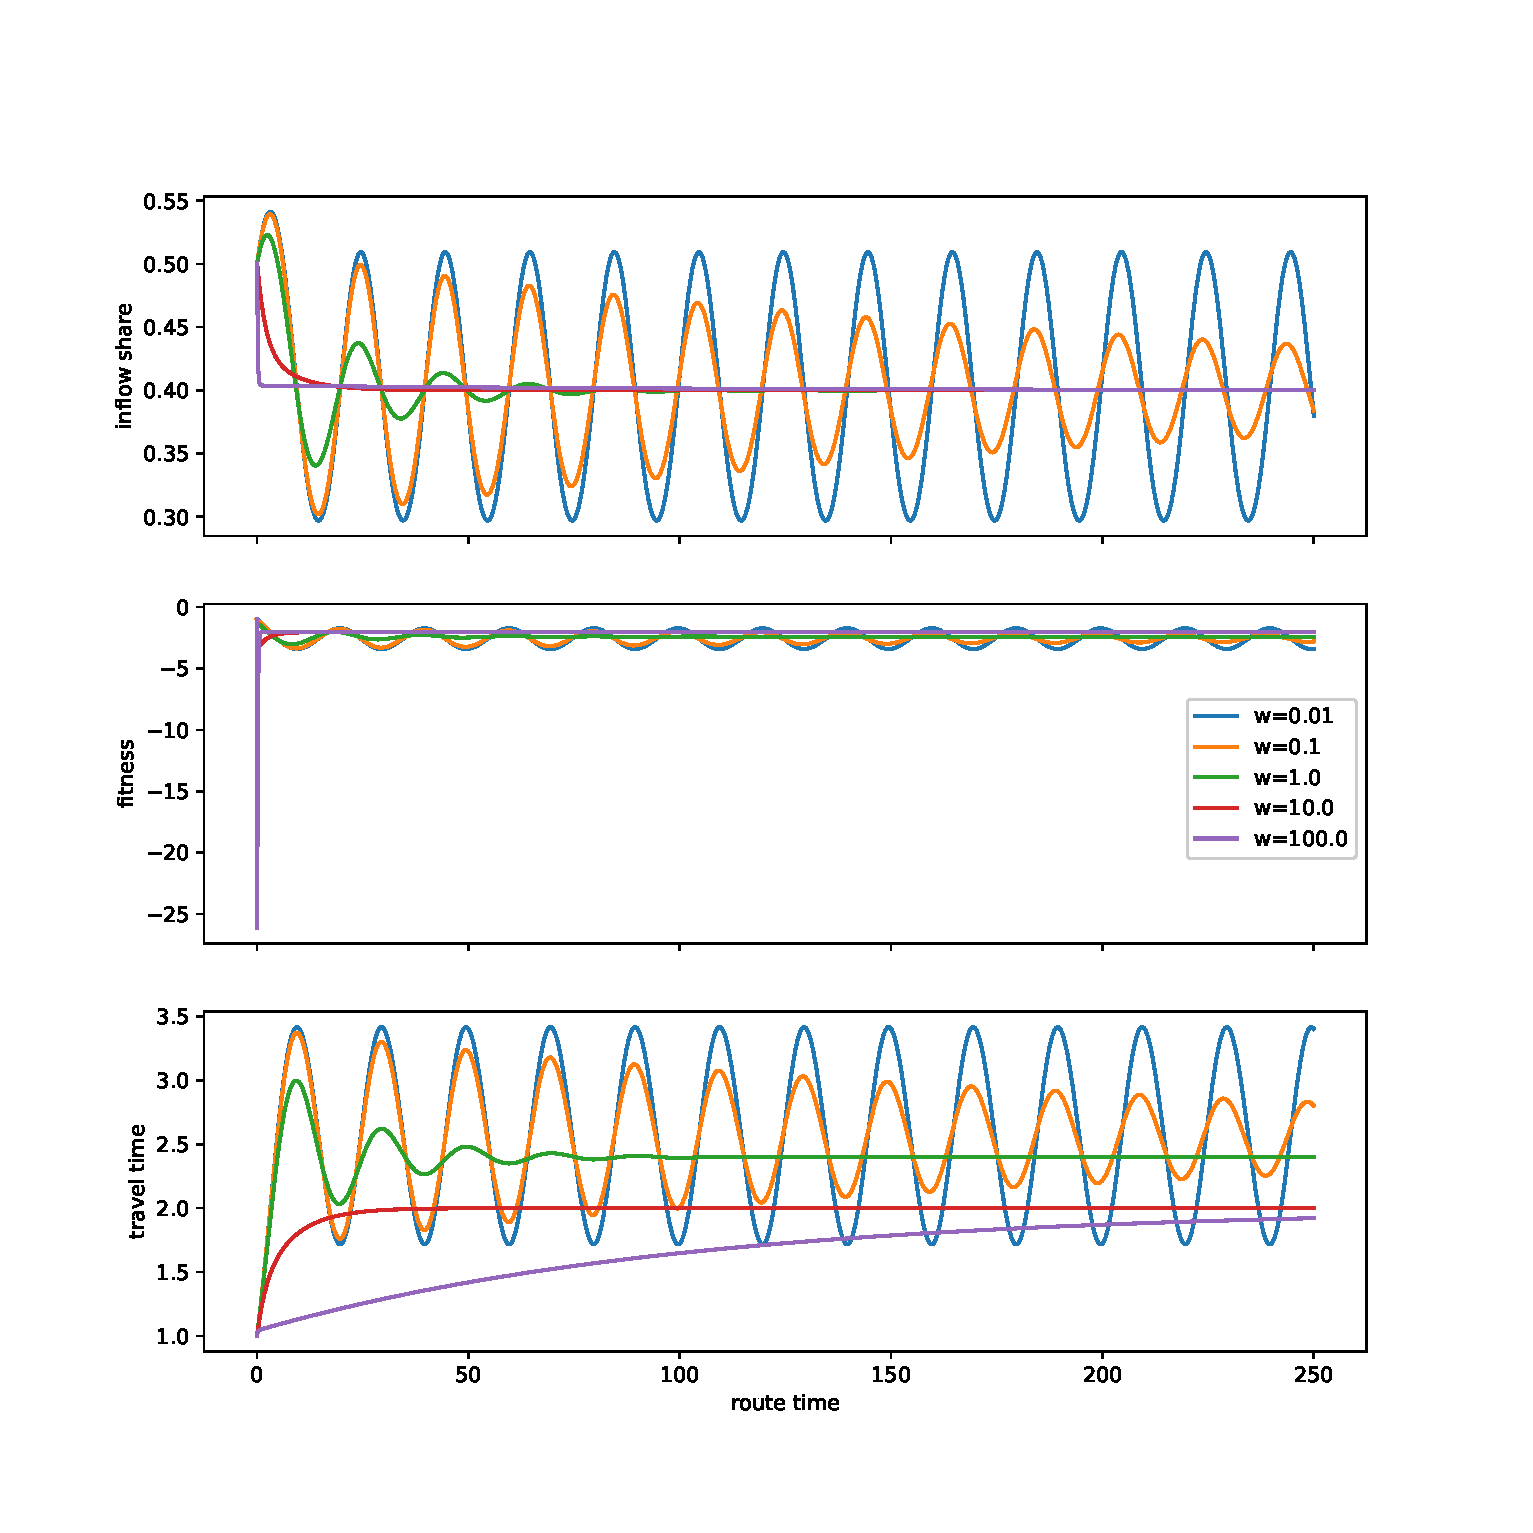
\includegraphics[width=0.9\textwidth]{img/replicator_proj_tt.eps}
	\caption{ $ U = 5, R=0.1, \Delta \theta = 0.01$}
	\label{fig:fluctuations_proj}

\end{figure}
	
\begin{figure}
	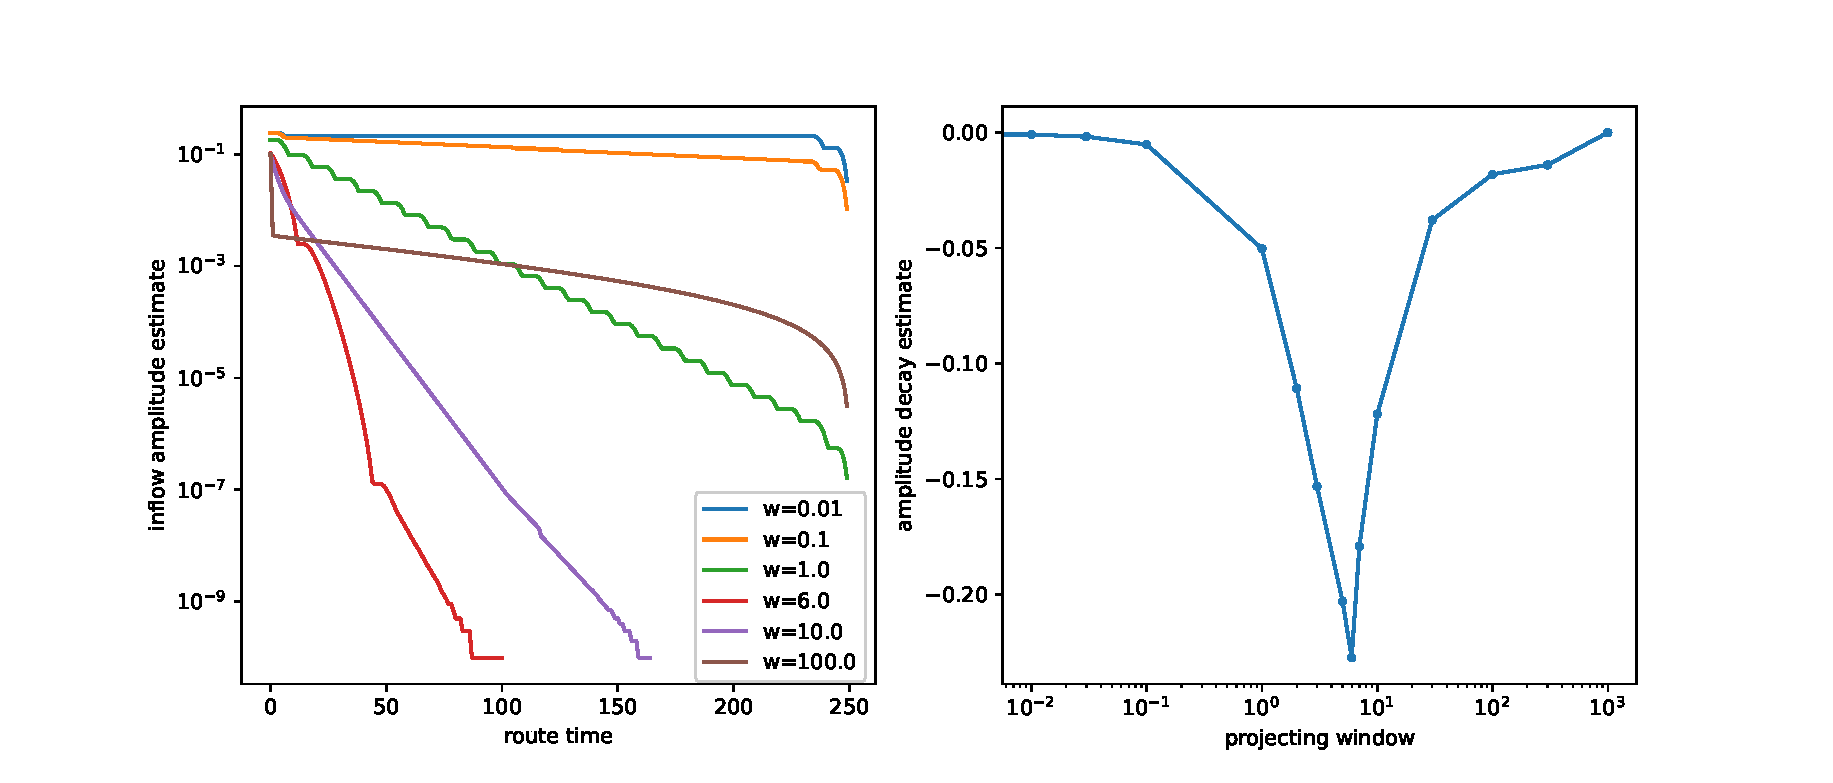
\includegraphics[width=0.9\textwidth]{img/amplitudes_proj_tt.eps}
	\caption{ Inflow amplitudes for path 0 }
	\label{fig:amplitudes_proj}

\end{figure}

\begin{figure}
	\includegraphics[width=0.9\textwidth]{img/final_tt_proj.eps}
	\caption{ Final travel times }
	\label{fig:final_tt_proj}

\end{figure}

%\begin{figure}
%	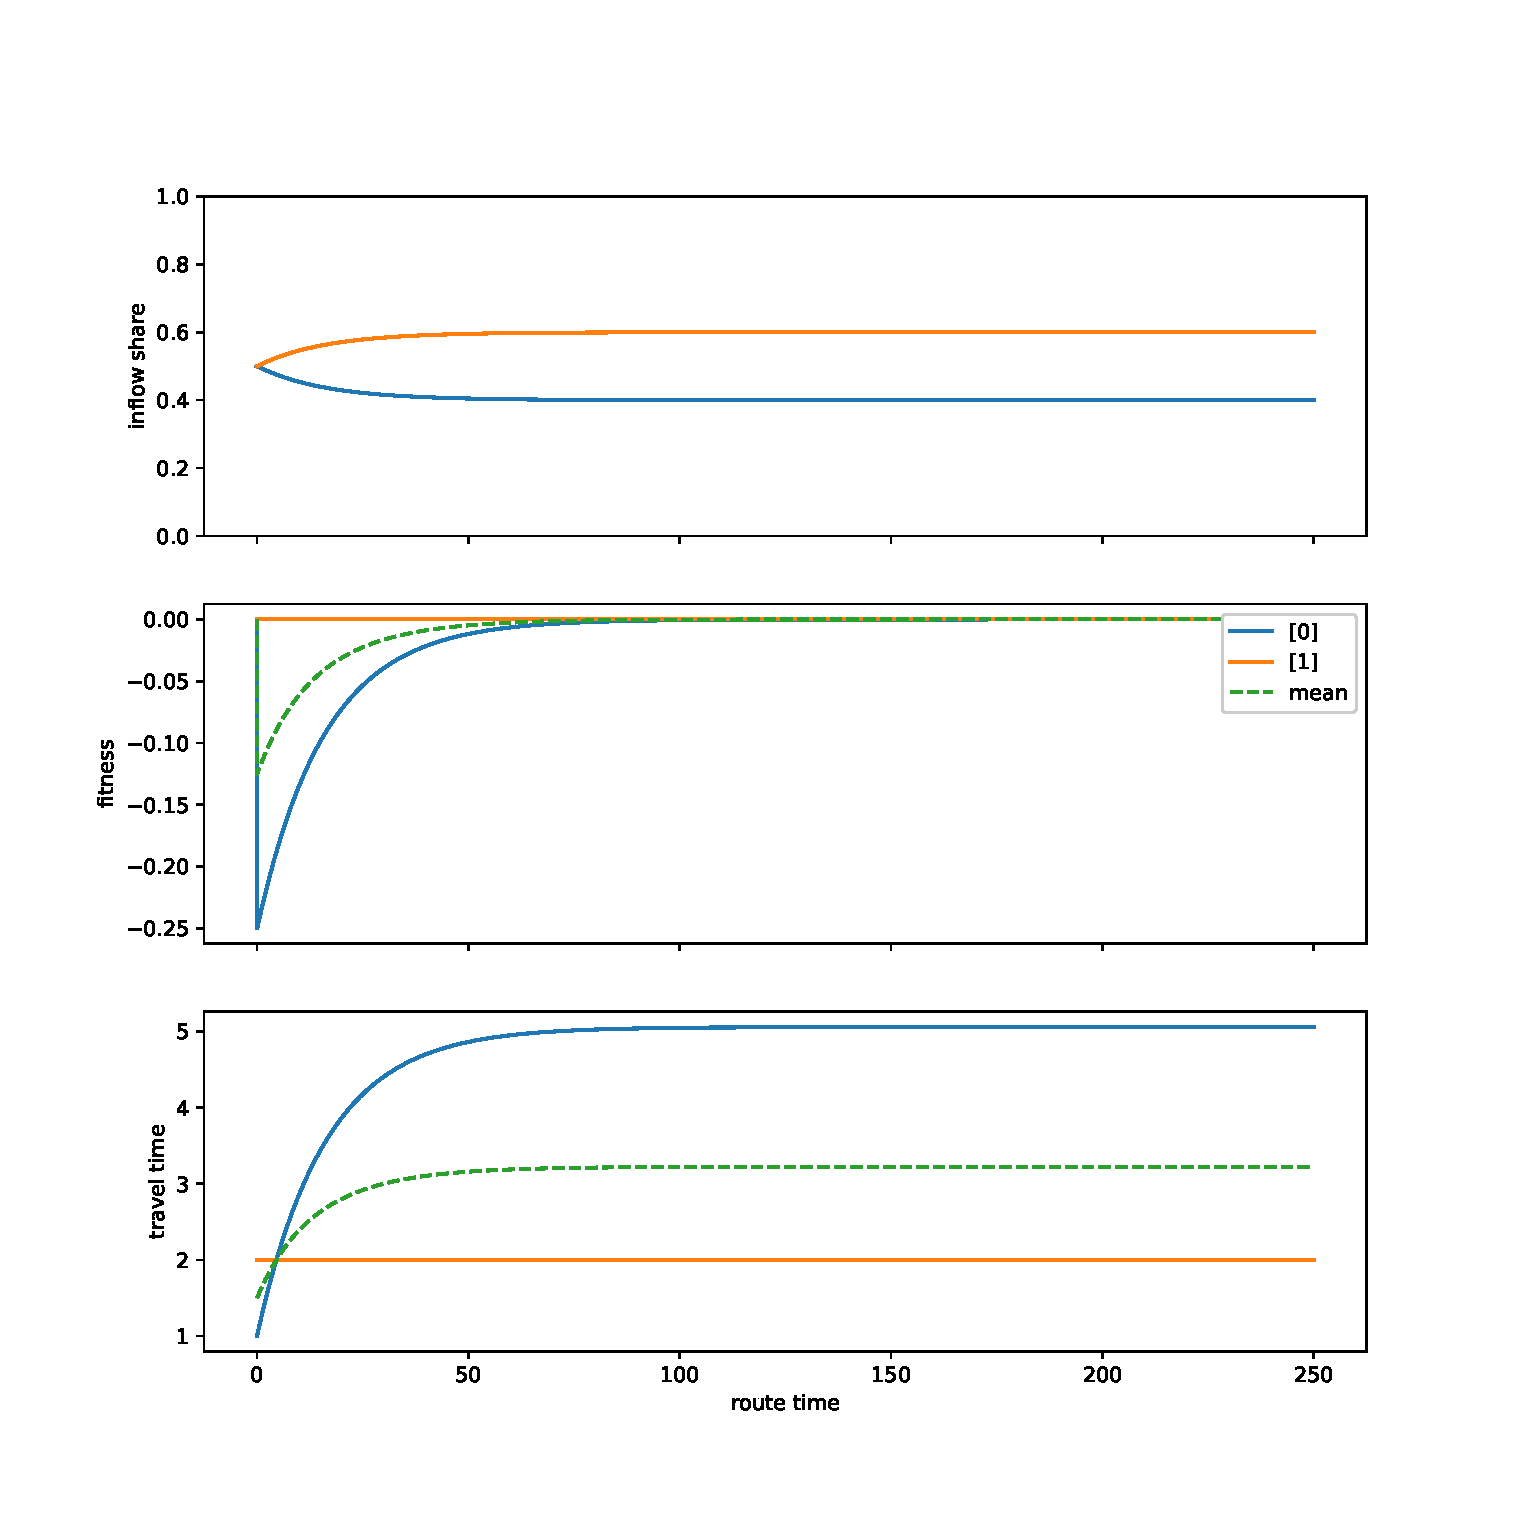
\includegraphics[width=0.9\textwidth]{img/replicator_grad_tt.eps}
%	\caption{ Travel time gradient as fitness }
%	\label{fig:replicator_grad_tt}
%
%\end{figure}

\newpage
\subsubsection*{Medium Demand ($ \nu_0 < U < \nu_0 + \nu_1$)}

Different cases have different equilibria:
$$ \frac{\nu_0}{U} > \frac{\nu_0}{\nu_0 + \nu_1} > \frac{U - \nu_1}{U}$$

Figure \ref{fig:case_switching} shows how cases switch until amplitude drops enough and we end up in case $q_0 > 0, q_1 = 0$.

Figure \ref{fig:replicator_medium_demand} shows dynamics for the faster edge 0 with different projection windows. 
Both fitnesses eventually stabilize to values $\phi = -\tau_1$ (negative cost of slower edge).
%It also appears that the queue doesn't form on edge 1, so it has constant fitness $\phi_1(\theta) \equiv - \tau_1 $.

\begin{figure}
	\includegraphics[width=0.9\textwidth]{img/case_switching.pdf}
	\caption{ Case switching }
	\label{fig:case_switching}
\end{figure}


\begin{figure}
	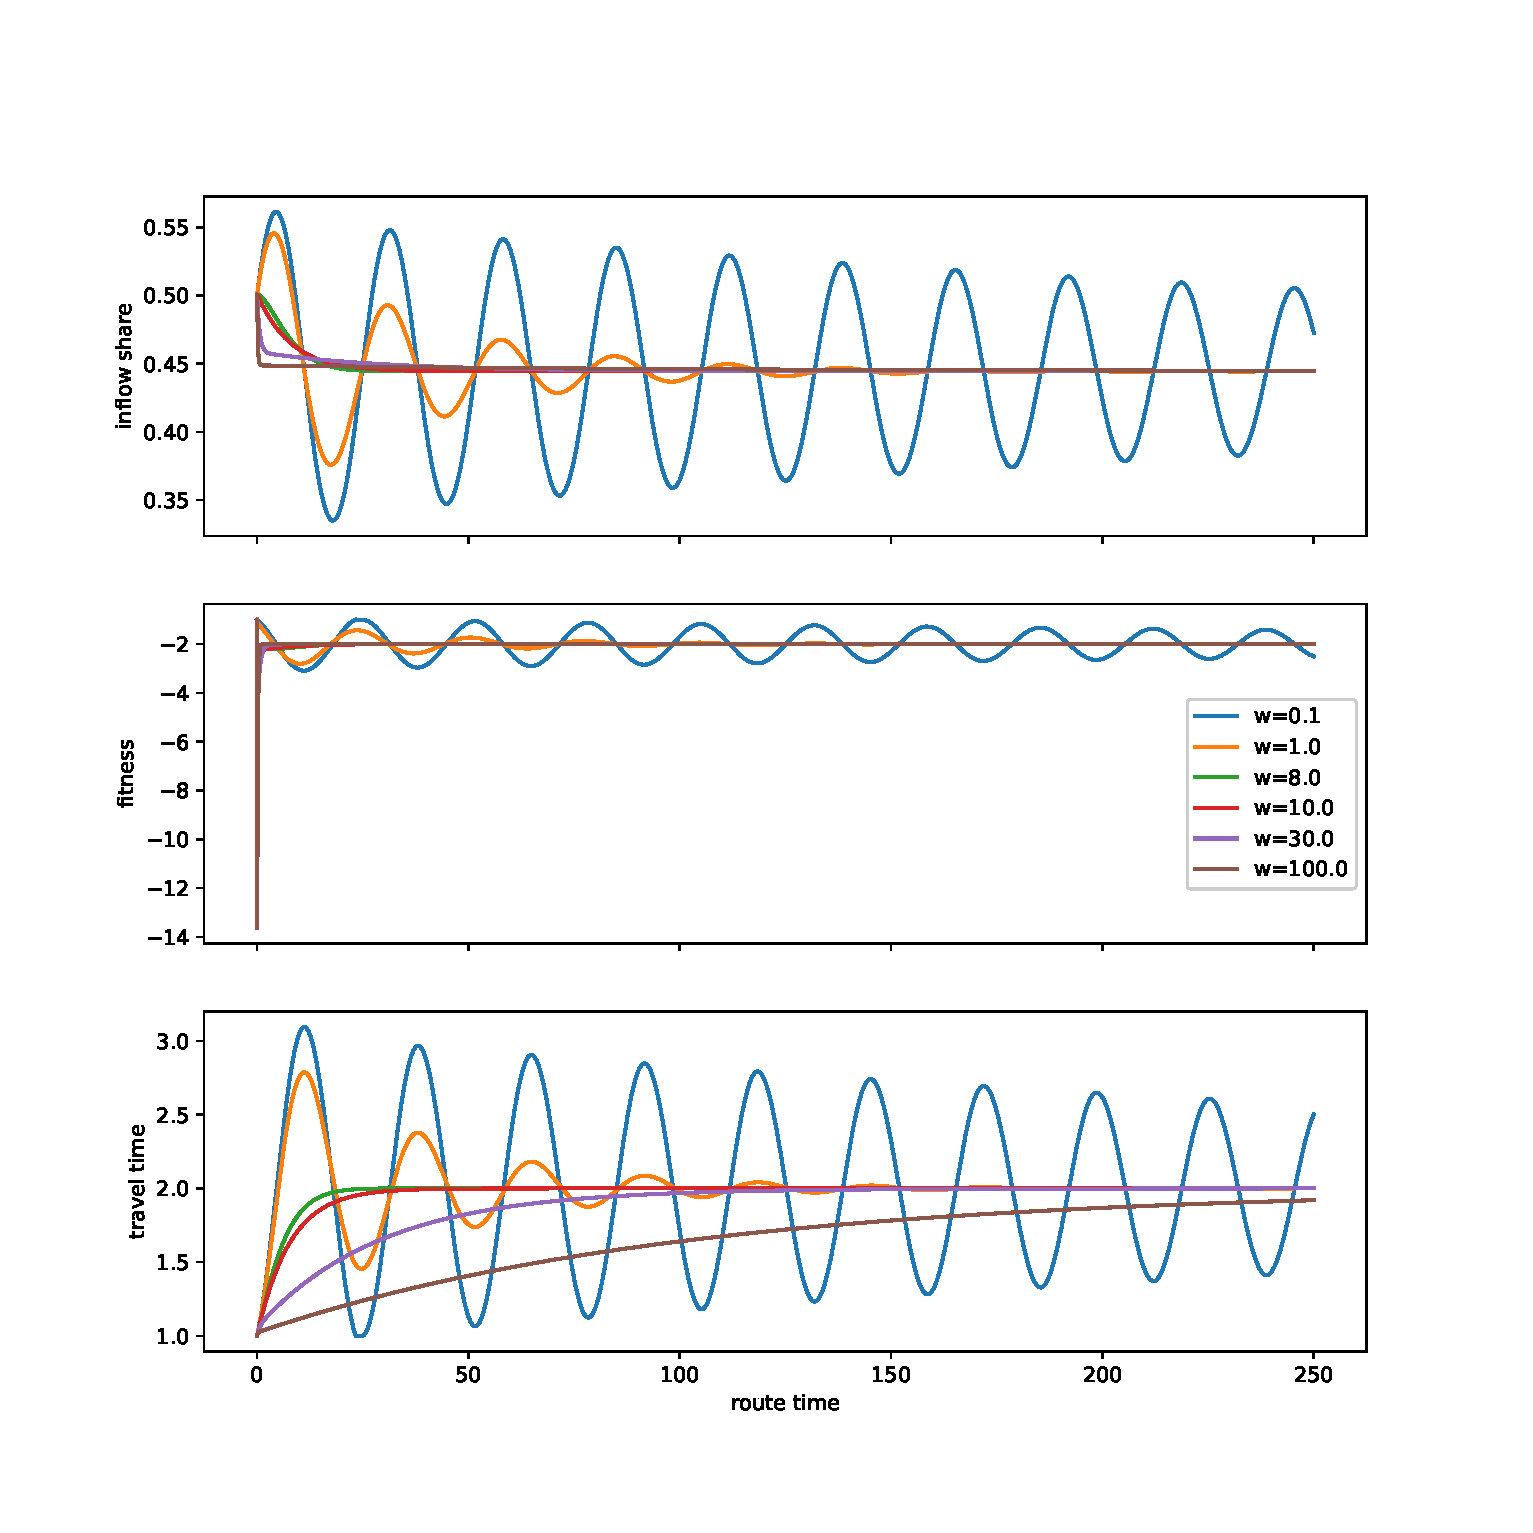
\includegraphics[width=0.9\textwidth]{img/replicator_medium_demand.eps}
	\caption{ Medium demand. $U = 4.5; \Delta\theta = 0.01; R = 0.1$ }
	\label{fig:replicator_medium_demand}

\end{figure}

Now assume that edge 0 operates on full capacity and  edge 1 always operates below capacity, i.e.

$$\dot{t_0}(\theta) = \frac{U\cdot h_0(\theta) - \nu_0}{\nu_0}, \quad
 \dot{t_1}(\theta) \equiv 0 .$$

%This  allows to write the replication equation
%$$ \dot{h}_0 = R \cdot h_0 \cdot (\phi_0 - h_0\phi_0 - (1-h_0)\phi_1) = -R \cdot h_0 \cdot ( 1- h_0 ) \cdot \left( \tau_0 + \frac{1}{\nu_0} (q_0 + w \cdot \frac{\partial q_0}{\partial \theta}) - \tau_1 \right) $$
%in the form
%$$ \ddot{\Phi} = - R \cdot (\Phi + w \dot{\Phi}) \cdot  (1+ \dot{\Phi}) \cdot (1 -  h^* (1+ \dot{\Phi})),$$
% where the following notation is used: 
% $$h^* := \frac{\nu_0}{U}, \quad \Phi(\theta) := t_0(\theta) - t_1(\theta) = \int_0^{\theta} \frac{h_0(z) - h^*}{h^*} dz + \tau_0  - \tau_1 .$$
%  We have $ h_0(\theta) = h^* (1 + \dot{\Phi}(\theta))$ and the assumptions can be written as 
Sufficient conditions of the solution to fulfill the assumptions:
 $$\Phi(\theta) - \Phi(0) \geq 0; \quad \dot{\Phi}(\theta) \geq  - \frac{ \nu_0 + \nu_1 - U}{\nu_0} .$$

%If we further assume that $\dot{\Phi}$ is small (i.e. $h_0$ is close to $h^*$), we can make a simplification and analyze the linear equation
%$$ \ddot{F} = - R \cdot(F + w \dot{F}) \cdot (1-h^*) \quad \Leftrightarrow \quad \ddot{F} + kw\dot{F} + kF = 0 , \quad k = R(1-h^*).$$
%
%This yields a theoretical estimate of decay rate:
%$$ w \leq \frac{2}{\sqrt{k}}: \quad h_0 - h^* \propto e^{-\frac{kw}{2} \theta}$$ 
%$$w > \frac{2}{\sqrt{k}}: \quad h_0 - h^* \propto e^{-\frac{kw - \sqrt{(kw)^2 - 4k}}{2}\theta}$$

Figure \ref{fig:amplitudes_decay} shows that that theoretical decay estimate is good.

\begin{figure}
	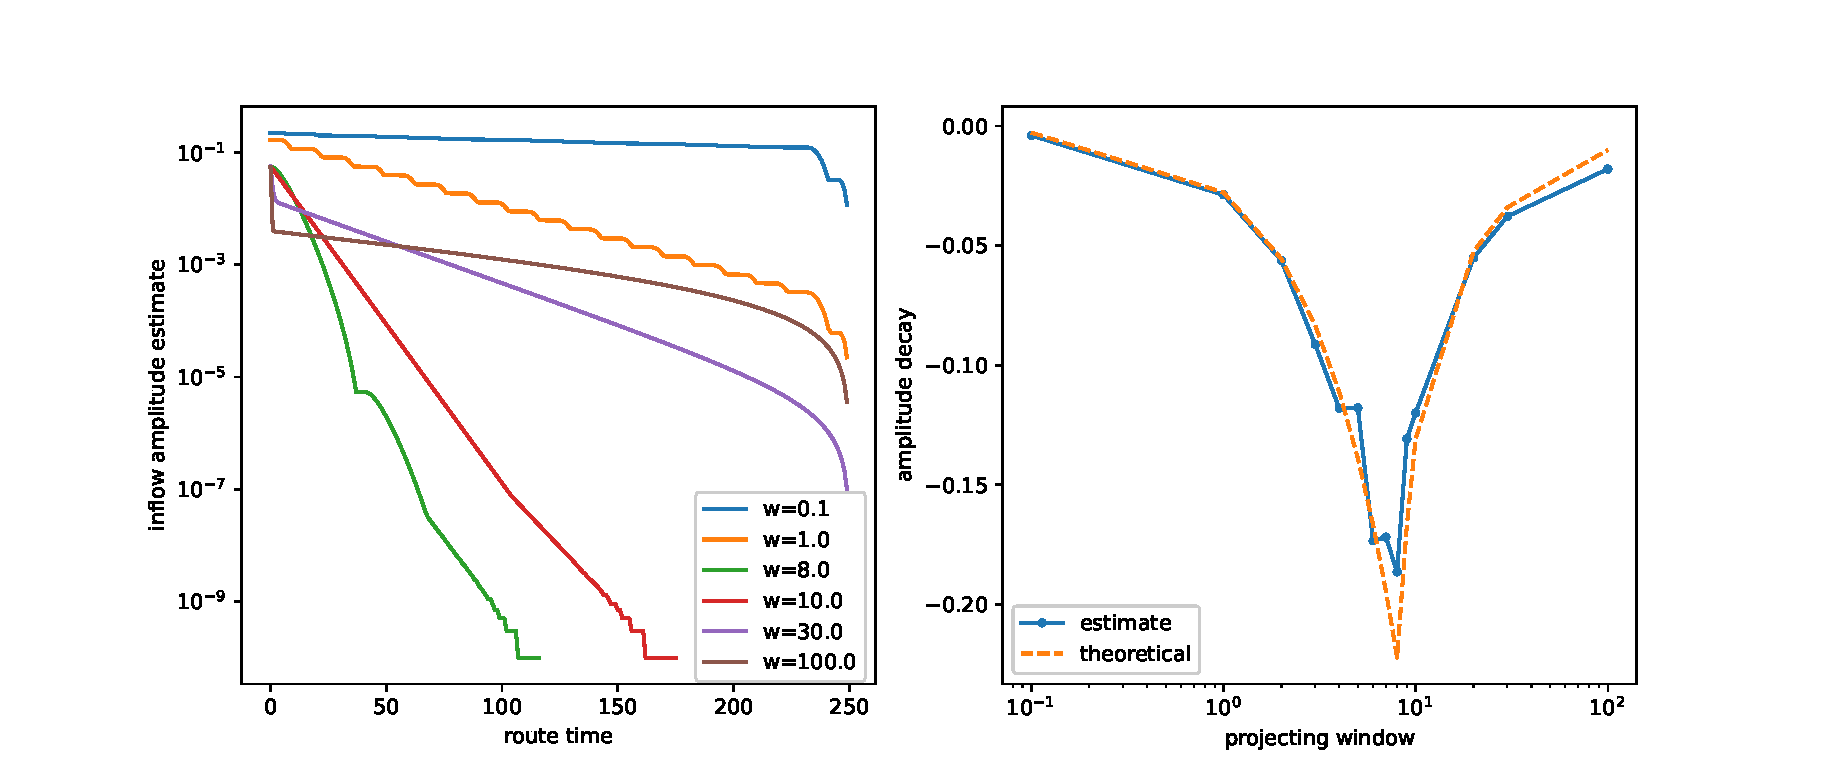
\includegraphics[scale=0.5]{img/amplitudes_decay.eps}
	\caption{Amplitudes decay }
	\label{fig:amplitudes_decay}

\end{figure}	

Figure \ref{fig:de_comparison} shows the difference between theoretical and observed dynamics. Used parameters: $ U = 4.5; \Delta\theta = 0.01;  h_0(0) = 0.5;  R = 0.1; w = 1.0 $

\begin{figure}
	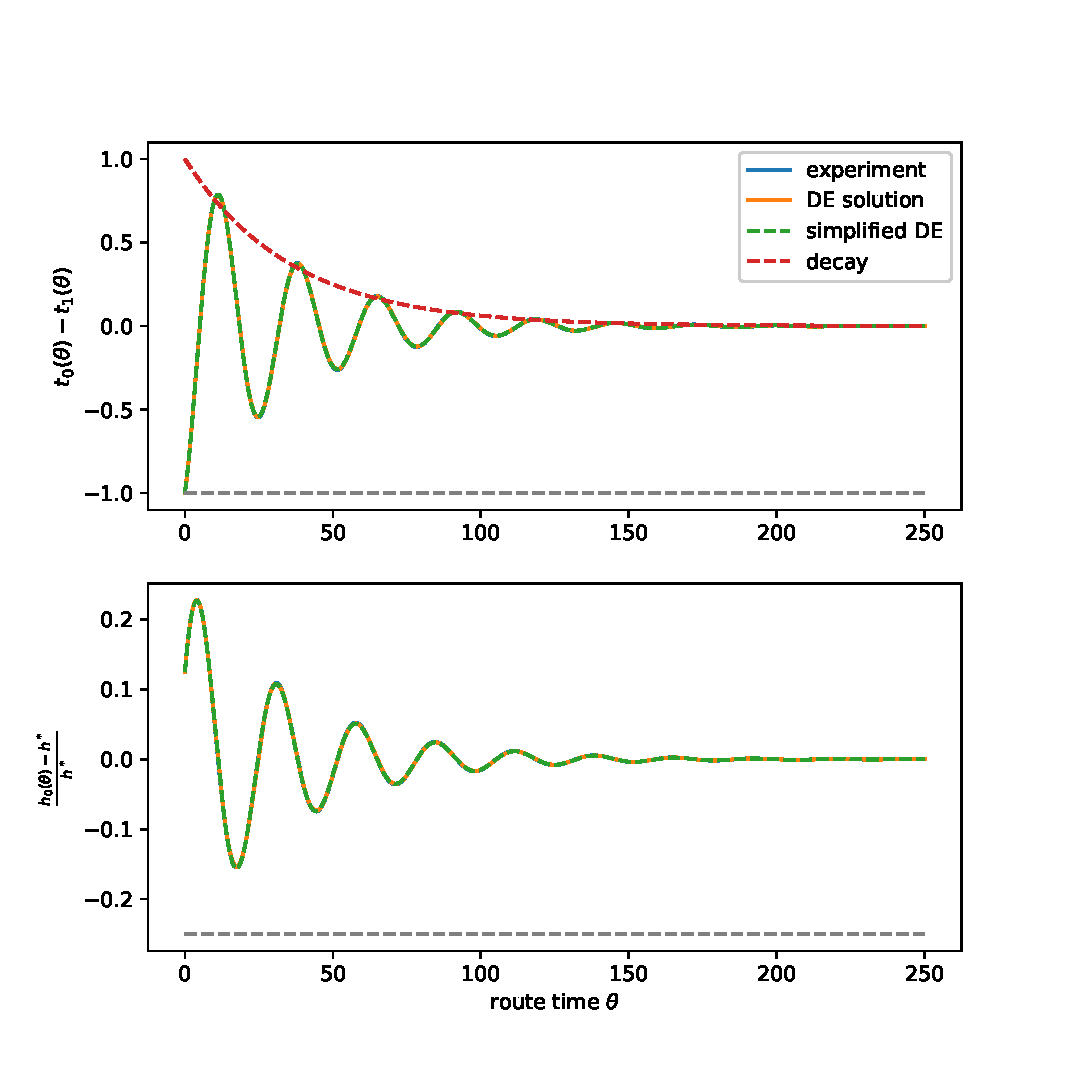
\includegraphics[scale=0.75]{img/de_comparison.eps}
	\caption{Solution of DEs compared to the experiment; gray dashed lines show illustrate fulfillment of assumptions }
	\label{fig:de_comparison}

\end{figure}	

Figures \ref{fig:replicator_inits_w_1} and \ref{fig:replicator_inits_w_opt} show dynamics for edge 0 with parameters $U = 4.5; \Delta\theta = 0.01; R = 0.1$ for different initial share with $ w = 1.0 $ and $w = \frac{2}{\sqrt{k}} = 8.49$

\begin{figure}
	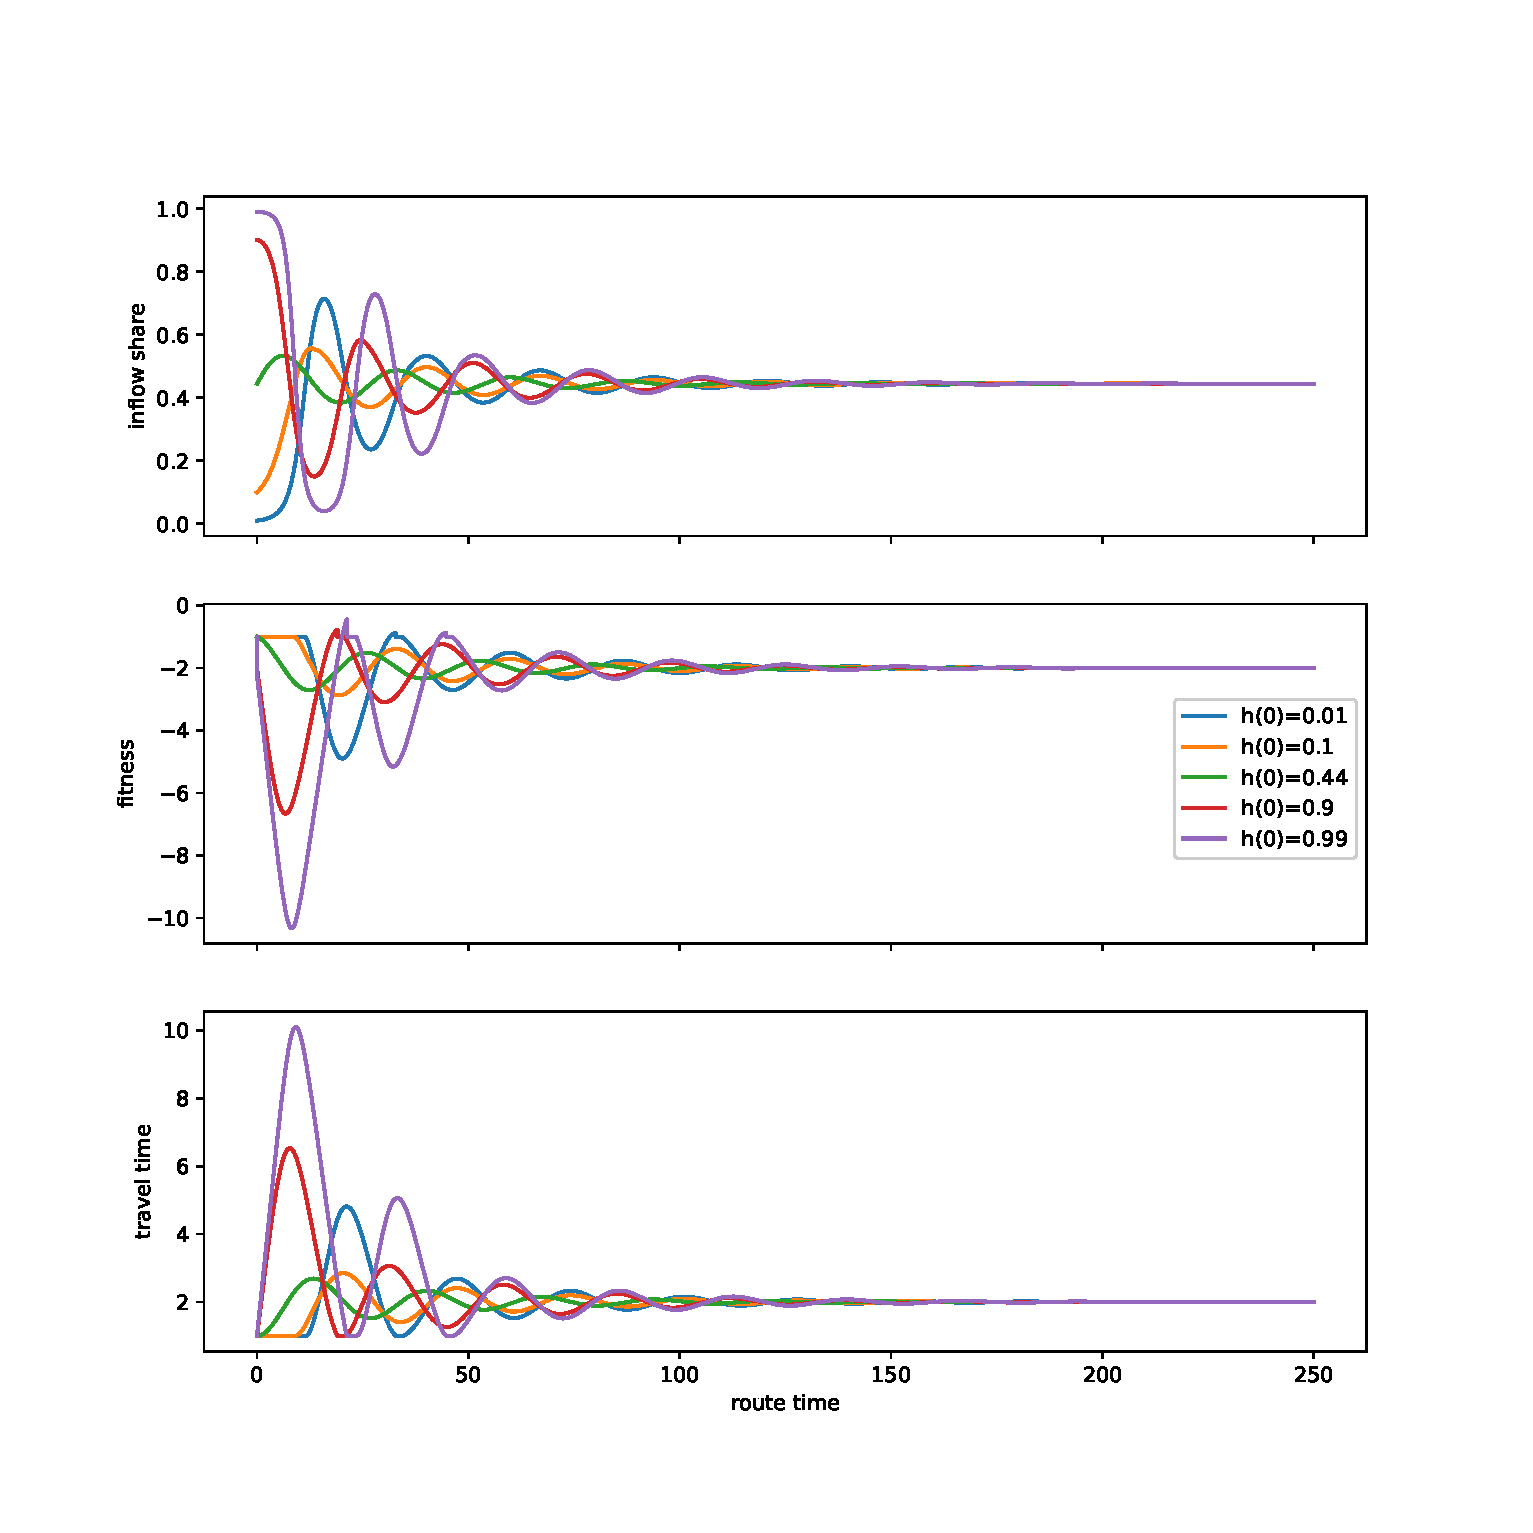
\includegraphics[scale=0.5]{img/replicator_inits_w_1.eps}
	\caption{ $ w = 1.0 $ }
	\label{fig:replicator_inits_w_1}

\end{figure}	

\begin{figure}
	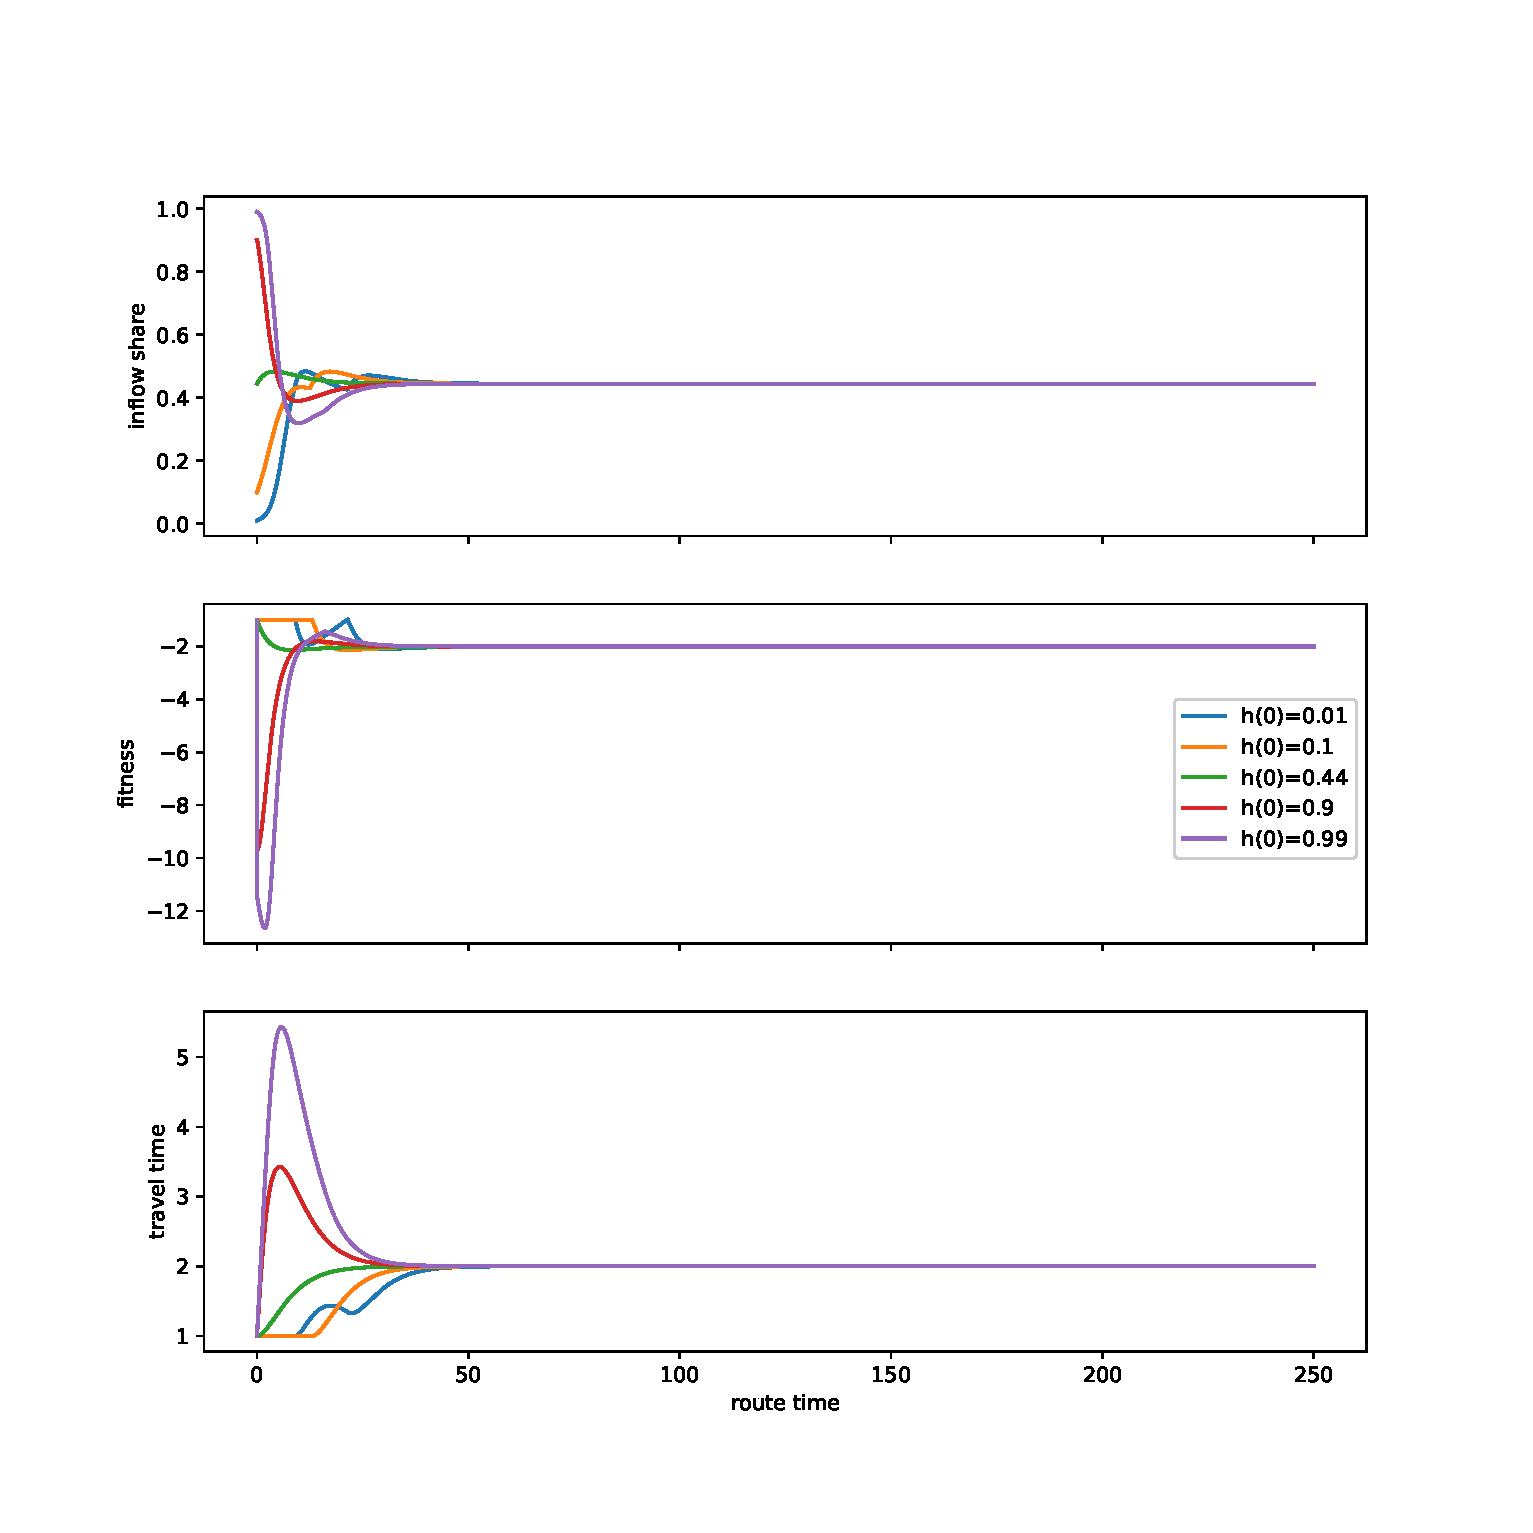
\includegraphics[scale=0.5]{img/replicator_inits_w_opt.eps}
	\caption{ $w = \frac{2}{\sqrt{k}} = 8.49$ }
	\label{fig:replicator_inits_w_opt}

\end{figure}	

%\subsection*{Sufficient conditions for convergence}
%
%Suppose we are in case 2 of medium demand setting and assume inflow rate always stays in the neighbourhood of $h^* = \frac{\nu_0}{U}$:
%$$ |h_0(\theta) - h^* | \leq | \frac{\nu_0}{U} - (1 - \frac{\nu_1}{U}) |= \frac{\nu_0 + \nu_1 - U}{U} .$$
%This guarantees no cases switching, as $U (1 - h_0(\theta)) \leq \nu_1$.   
%\\
%Denote $ m := \min_{\theta} h_0(\theta)(1 - h_0(\theta)) > 0 $
%\\
%Consider $V(\Phi, \dot{\Phi}) = \Phi^2 + (\Phi + w \dot{\Phi}) ^2 >0 $.
%$$ \dot{V} = \frac{\partial V}{\partial \Phi} \dot{\Phi} + \frac{\partial V}{\partial \dot{\Phi}} \cdot \left( -\frac{R}{h^*} h_0(1-h_0)(\Phi + w \dot{\Phi}) \right)  = $$
%$$ = \left( 4\Phi\dot{\Phi} + 2w\dot{\Phi}^2 \right) - 2w \frac{R}{h^*} h_0(1-h_0)(\Phi + w \dot{\Phi})^2 \leq \left(  4\Phi\dot{\Phi} + 2w\dot{\Phi}^2 \right) - 2w\frac{Rm}{h^*} (\Phi + w \dot{\Phi})^2 = $$
%$$ = 2w \left( \frac{1}{w^2} - \frac{Rm}{h^*} \right)  (\Phi + w \dot{\Phi})^2 - \frac{2}{w} \Phi^2  .$$
%\\
%We can guarantee $\dot{V} < 0$ for $w \geq \sqrt{\frac{h^*}{Rm}}$. With used parameters that is:
%$$w \geq \sqrt{ \frac{ 2/4.5 }{ 0.1 \cdot 3/4.5 \cdot (1-3/4.5)} } \approx 4.47 .$$


\newpage
\subsection*{Unstable dynamics}

Figures \ref{fig:fluctuations_avg}, \ref{fig:fluctuations_last} and \ref{fig:fluctuations_pred} show how using bad fitness leads to divergence.

\begin{center}
	\begin{figure}
	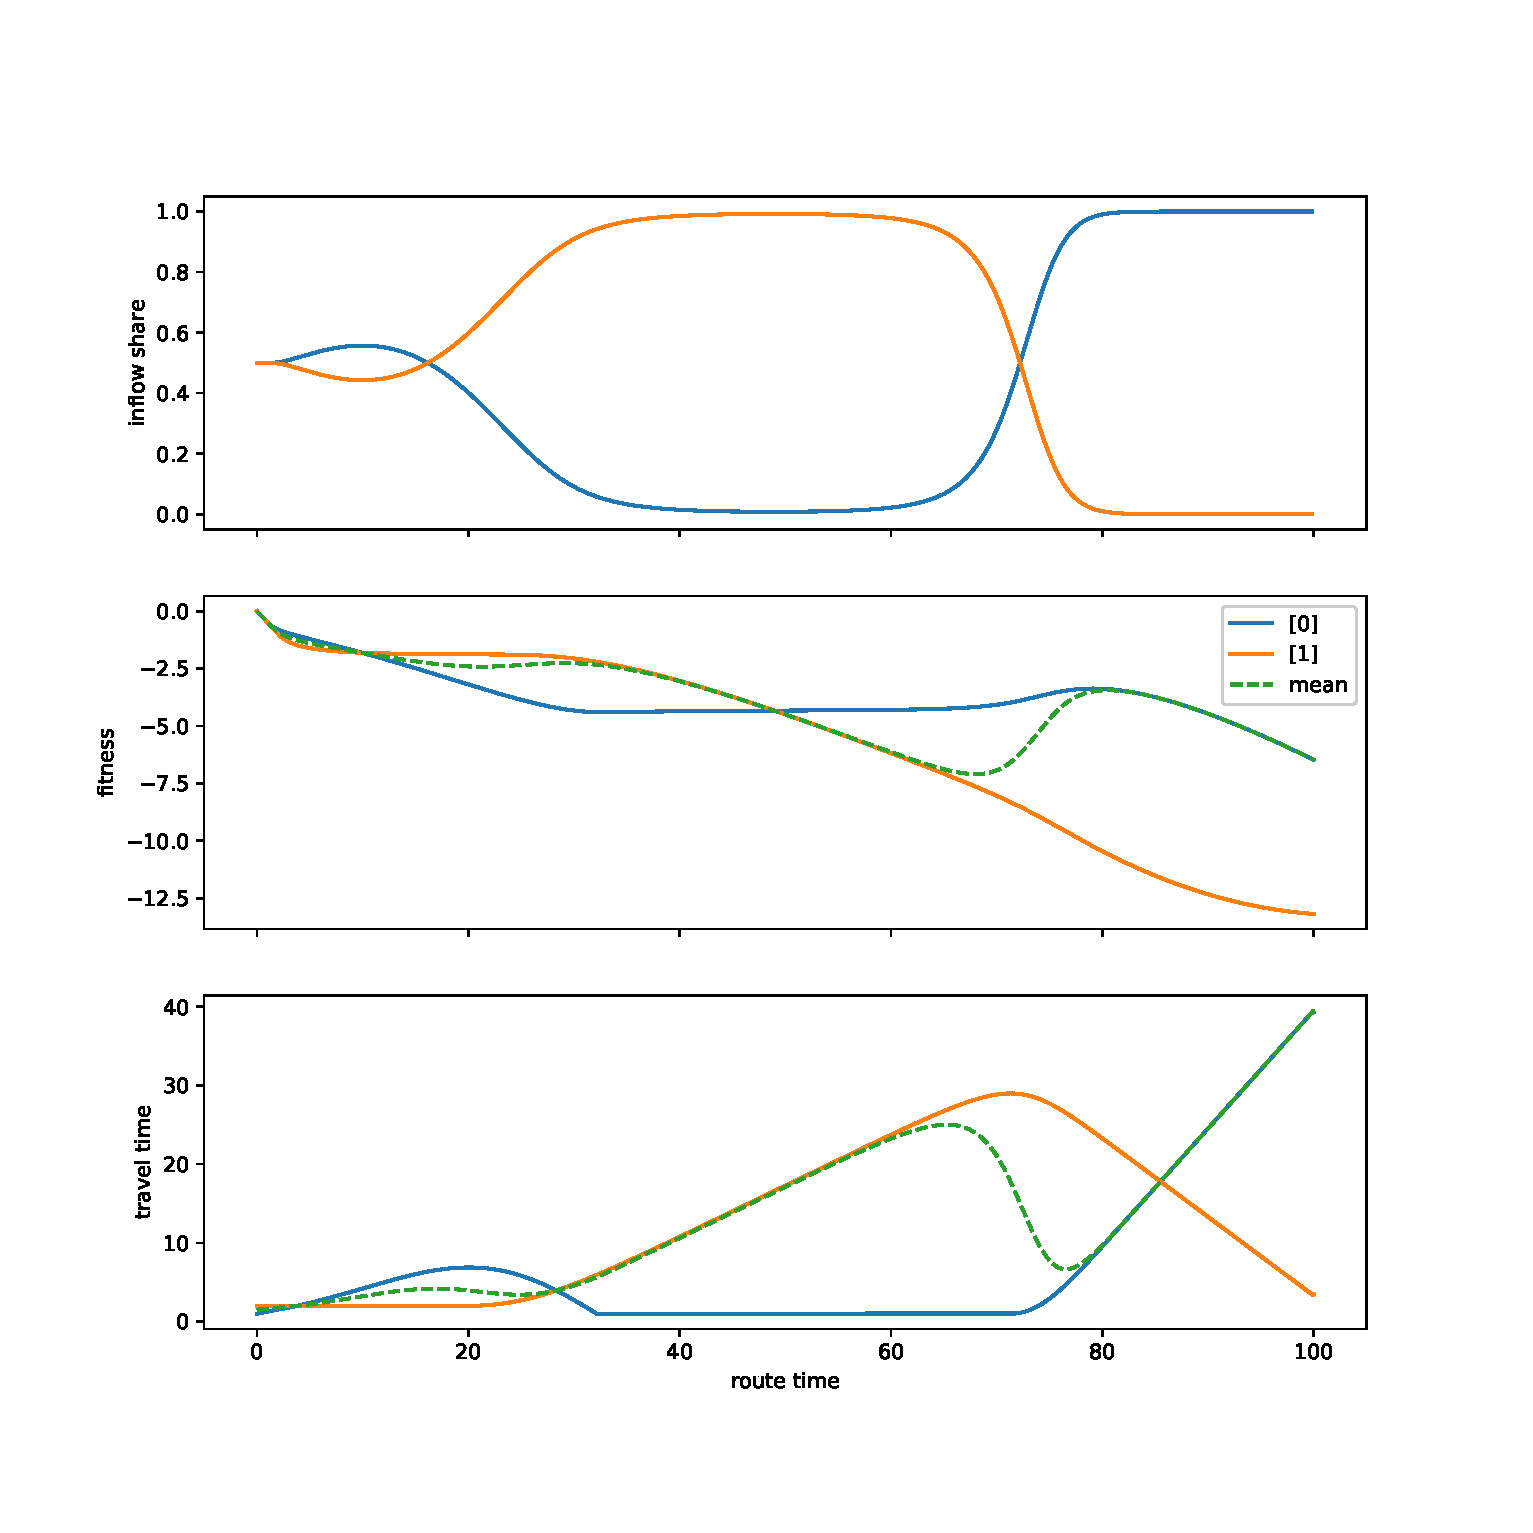
\includegraphics[scale=0.5]{img/replicator_avg_tt.eps}
	\caption{Fluctuations, average travel time }
	\label{fig:fluctuations_avg}

	\end{figure}
	
\end{center}

\begin{center}
	\begin{figure}
	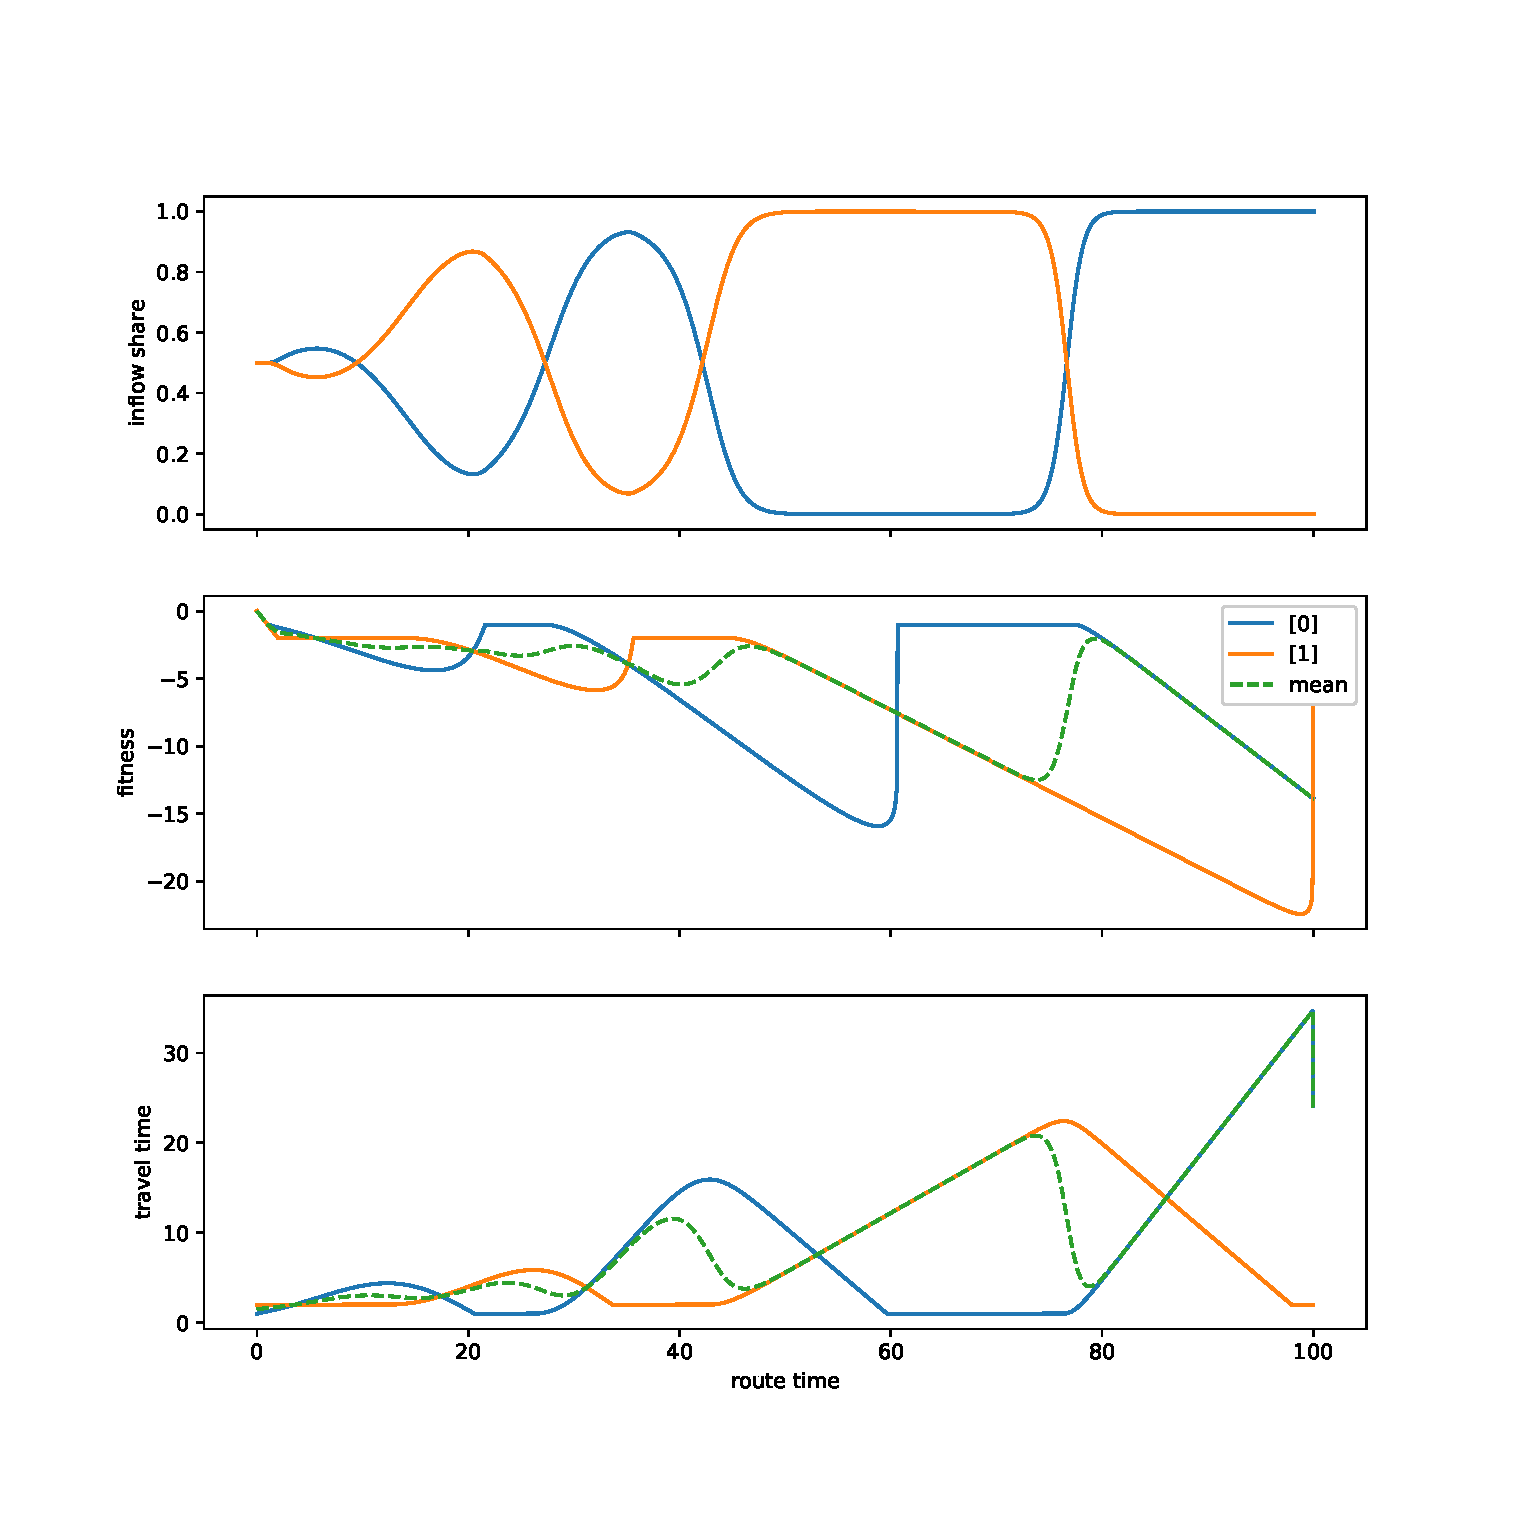
\includegraphics[scale=0.5]{img/replicator_last_tt.eps}
	\caption{Fluctuations, last travel time }
	\label{fig:fluctuations_last}

	\end{figure}
	
\end{center}

\begin{center}
	\begin{figure}
	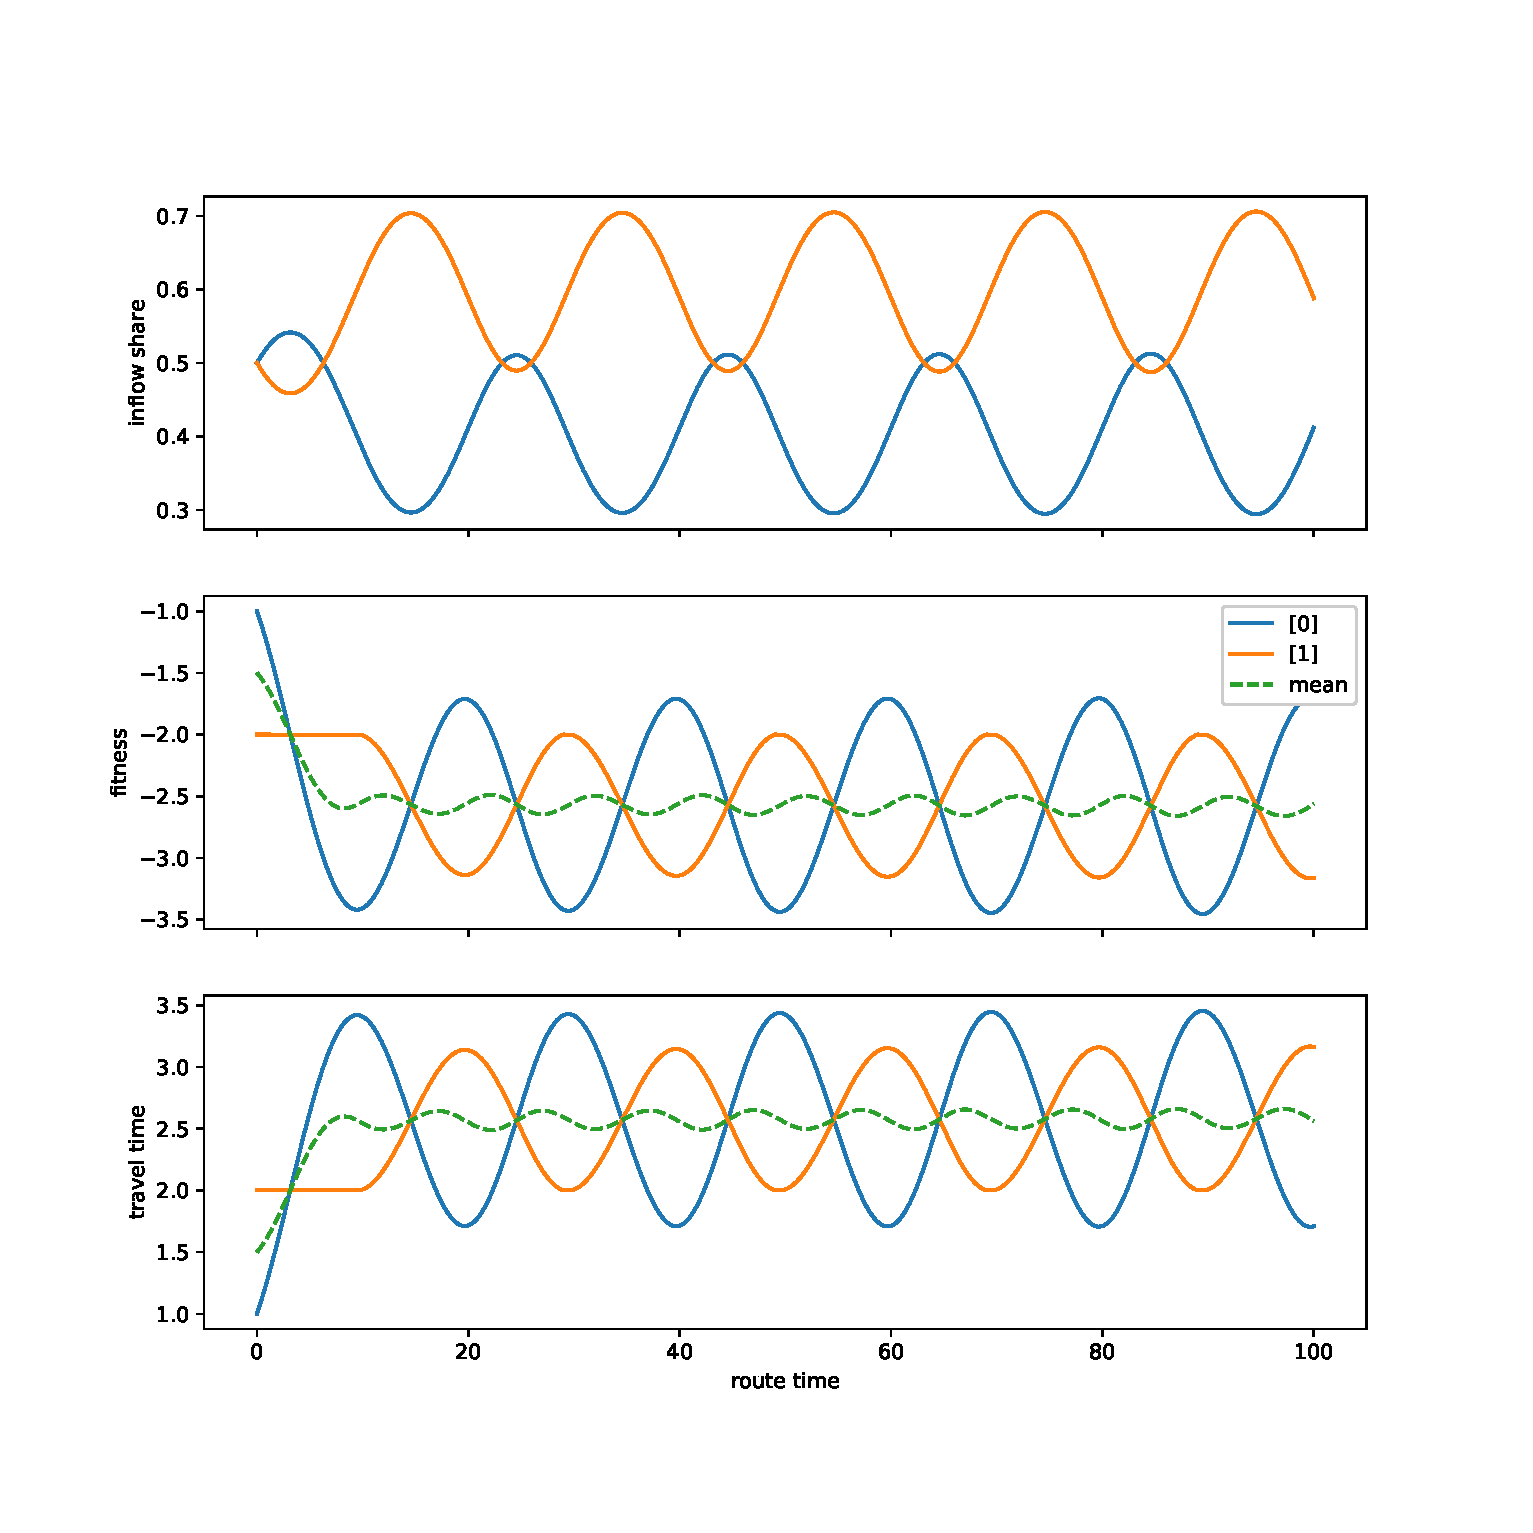
\includegraphics[scale=0.5]{img/replicator_pred_tt.eps}
	\caption{Fluctuations, predicted travel time }
	\label{fig:fluctuations_pred}

	\end{figure}
	
\end{center}

\subsubsection*{Proof ?}

Necessary condition for stability: $ \forall P: ~ \phi_P(\theta, h) = \sum_{P'} h_{P'}(\theta) \phi_{P'}(\theta, h) $. \\
In cases of average travel time and last travel, influence of inflows on fitnesses is delayed for at least $\tau_0$. \\ 

Sufficient condition for stability for non-aggregated travel times: queues have to not change for the period of delay. This guarantees that fitnesses don't change once equality is reached.
\\

Even when we use undelayed travel times, inflows tend to get in antiphase with fitnesses.
In this example, we need inflows to equalize with edge capacities at the moment when both path have same costs.


\end{document}